\chapter{Literature Review}  \label{cha Literature Review}%Title of the First Chapter


 \graphicspath{{Figs/}}
 
 
% \iffalse

%REdraw case setup
%phrase banck manchester


This research investigates the interaction between fluid and multiple cylinders, which is most often placed in the context of multi-cylinder vortex-induced vibration (VIV). This literature review, therefore, lays emphasis on the vortex-induced vibration for both single and multiple cylinders.

Vortex-induced vibration (VIV) accounts for disastrous failures in various engineering applications, including aero, civil, mechanical, marine, offshore, and nuclear engineering. Ever since Leonardo da Vinci first observed VIV in 1504AD, in the form of  "Aeolian Tones," engineers have spared no effort on investigating VIV to mitigate its damaging effects \cite{vortexhydroenergy}. VIV of a bluff body exposed to a flow is a result of vortex formation and shedding on the downstream side the body. Vortex shedding alternates from one side to another, causing oscillations or even the torsional vibrations of elastic bodies (e.g. cylinders, spheres). This fluid-structure interaction phenomenon occurs as a result of lock-in, i.e. synchronisation between vortex shedding and bluff body oscillation, due to non-linear resonance of cylinders (or spheres). This chapter summarises the most significant research for single cylinder VIV, as well as that for multi-cylinder VIV. 

%In addition, the most disastrous VIV structure failure is the collapse of Tacoma Narrows Bridge in Washington State in 1940.

%********************************** %First Section  **************************************
\section{Vortex-induced Vibration of Single Cylinder} \label{sec:VIV1}%Section - 1.1 

This section discusses flow-induced vibration of a freely oscillating elastically mounted cylinder with 1-Degrees-Of-Freedom (1DOF). \Cref{table:non_dimensional_groups} lists the frequently used non-dimensional groups throughout this chapter.

%\subsection{Non-dimensional Groups}

\bgroup
\def\arraystretch{2.2}%row height stretching coefficient
	\begin{table}[h]
		\caption{Non-dimensional groups in literature review}
		\centering
		\label{table:non_dimensional_groups}
		\begin{tabular}{l c c }
			\toprule
	%		\multirow{2}{*}{Dental measurement} & \multicolumn{2}{c}{Species I} & \multicolumn{2}{c}{Species II} \\ 
	%		\cmidrule{2-5}
	%		& mean & SD  & mean & SD  \\ 
	%		\midrule
			Mass ratio & $\mr$ & {\Large $ \frac{m}{\pi \rho D^2 L /4} $}  \\
			
			Damping ratio (with added mass) & $  \dr $ &{\Large $ \frac{c}{2\sqrt{k(m+m_A)}} $ }\\
			
			Velocity ratio & $ \vr $&{\Large  $ \frac{U}{f_{wn} D} $}\\
			
			Amplitude ratio & $ \ar $ &{\Large $ \frac{A}{D} $  }\\
			
			Frequency ratio & $\fr$ &{\Large  $ \frac{f}{f_{wn}} $}\\
			
			Transverse force coefficient & $ \cy $&{\Large $ \frac{F}{0.5 \rho U^2DL} $}\\ 
	
			Reynolds number & $ Re $ &{\Large $ \frac{\rho UD}{\mu} $}\\
			\bottomrule
		\end{tabular}
	\end{table}
\egroup



\subsection{Classic equations for cylinder oscillation}
Several equations have been commonly used in the investigation of a cylinder's vortex-induced vibration (VIV), describing the motion of a cylinder and the forces upon it. \Cref{eq:1} is used to describe the motion of cylinder in the Y (transverse) direction:
\begin{equation}	\label{eq:1}
	m\ddot{y}+c\dot{y}+ky=F(t)
\end{equation}
where m is the mass of cylinder, y is the displacement of the body,  c is the structural damping coefficient, k is the spring's stiffness constant, and $F(t)$ is the time-dependent force induced by the surrounding fluid \cite{bearman1984}. Furthermore, it is common to rewrite \Cref{eq:1} as \Cref{eq:1a}:
\begin{equation}	\label{eq:1a}
	M\ddot{y}+4\pi f_n \zeta M \dot{y}+4{\pi}^2{f_n^2} M y=C_y \rho U^2 D /2
\end{equation}
where $M=m/L$ is the mass per unit span, $\zeta$ is the damping ratio, $f_n=(k/M)^{1/2} / 2\pi$ is the undamped natural frequency (also termed as "structural natural frequency" \cite{Zhao2013}), $C_y=F(t)/0.5 \rho U^2 D $ is the lift force coefficient (sometimes written as $C_L$ \cite{Zhao2013a}). $C_y$ reflects the transverse direction component of the resultant instantaneous fluid force upon the oscillating bluff body, and includes parts considered as damping forces and fluid inertia.

Furthermore, provided that synchronisation (lock-in) between vortex wake and the cylinder's oscillation occurs, \Cref{eq:2,eq:3} are suitable representations of the force coefficient ($C_y$) and the response ($y$):
\begin{equation}	\label{eq:2}
	C_y(t)=C_{y_0} sin(\omega t+\phi)
\end{equation}
\begin{equation}	\label{eq:3}
	y(t)=A sin(\omega t)
\end{equation}
where $\omega$ is equivalent to $2\pi f$ and $f$ is the actual frequency of cylinder's oscillation; $C_{y_0}$ and $A$ are the amplitude of force coefficient and body oscillation, respectively; and $\phi$ is the phase angle difference between force and body oscillation. 

\Cref{eq:4,eq:5} can be deducted from \Cref{eq:1a,eq:2,eq:3} (see \Cref{ap:deducequ} for details), as described by Bearman \cite{bearman1984}:
\begin{equation}	\label{eq:4}
	\frac{\fosc}{f_n}=[1-\frac{C_{y_0}}{4\pi^2}cos\phi\frac{\rho D^2}{2M}(\frac{U}{f_nD})^2\frac{D}{y}]^{1/2}=\sqrt{\frac{m^*}{m^*+C_{EA}}}
\end{equation}
\begin{equation}	\label{eq:5}
%\frac{A}{D}=\frac{C_{y_0}}{8 \pi ^2}  \frac{ \rho D^2}{2M \zeta}  \frac{f_n}{f}  (\frac{U}{f_nD})^2  sin \phi
\frac{A}{D}=\frac{1}{4 \pi ^3}  \frac{ C_{y_0} sin \phi}{m^* \zeta} (\frac{U}{fD})^2 \frac{\fosc}{f_{n}}
\end{equation}
while Williamson \cite{Williamson2004} transformed \Cref{eq:4,eq:5} into \Cref{eq:6a,eq:6} by the fact that $ f_{wn}/f_n=\sqrt{m^*/(m^*+C_A)} $:
%\begin{equation}	\label{eq:6b}
%f_{wn}=\sqrt{\frac{m^*+C_A}{m^*+C_{EA}}}
%\end{equation}
\begin{equation}	\label{eq:6a}
f^*=\frac{\fosc}{f_{wn}}=\sqrt{\frac{m^*+C_A}{m^*+C_{EA}}}
\end{equation}
\begin{equation}	\label{eq:6}
A^*=\frac{A}{D}=\frac{1}{4 \pi ^3}  \frac{ C_{y_0} sin \phi}{(m^* + C_A)\zeta} (\frac{U}{fD})^2 \frac{\fosc}{f_{wn}}
\end{equation}
where $C_{EA}$ is the effective added mass coefficient as seen in \Cref{eq:7}:
\begin{equation}	\label{eq:7}
C_{EA}=\frac{1}{2 \pi ^3}  \frac{ C_{y_0} cos \phi}{A/D} (\frac{U}{\fosc D})^2 
\end{equation}

The form of \Cref{eq:6a,eq:6} is slightly different from \Cref{eq:4,eq:5} in that the added mass, $C_A$, is utilised ($C_A\approx1.0$ for a circular cylinder), and the undamped natural frequency (in vacuum) $f_n$ is replaced by the natural frequency in still water ($f_{wn}$). %This adjustment should yield better prediction results as it is a more precise approximation of the engineering reality. 
%CHECK Above sentence

Moreover, some issues were encountered with the application of added mass $m_A$ and the natural frequency $ f_n $ in these equations. The true natural frequency $ f_{n,true} $ is actually not a constant but varies according to the fluid added mass of the oscillating cylinder \cite{VIKESTAD2000}: $f_{n,true} \xrightarrow{depends \,\,\, on }m_A$. The oscillation frequency $ \fosc $, and therefore probably also $m_A$, is known to depend on reduced velocity $ \vr=U/f_nD $, for cylinders with low mass ratio\cite{Sarpkaya1979}: $m_A \xrightarrow{depends \,\,\, on} f_{osc} \xrightarrow{depends \,\,\, on} \vr \xrightarrow{depends \,\,\, on} f_{n,true} $. As we can see, here emerges a circular problem which is usually solved by predefining the value of $ f_n $. For example, it is often prescribed as the natural frequency measured in still water $ f_{wn }$ \cite{Williamson2004,VIKESTAD2000}, corresponding to $ C_A(f_{wn })=1.04 $.

\begin{figure}[tbp]	
	\centering
	%\captionsetup[subfigure]{labelsep = none}
	%\captionsetup[subfigure]{labelformat = empty}
	\begin{subfigure}[t]{\linewidth}
		\centering
		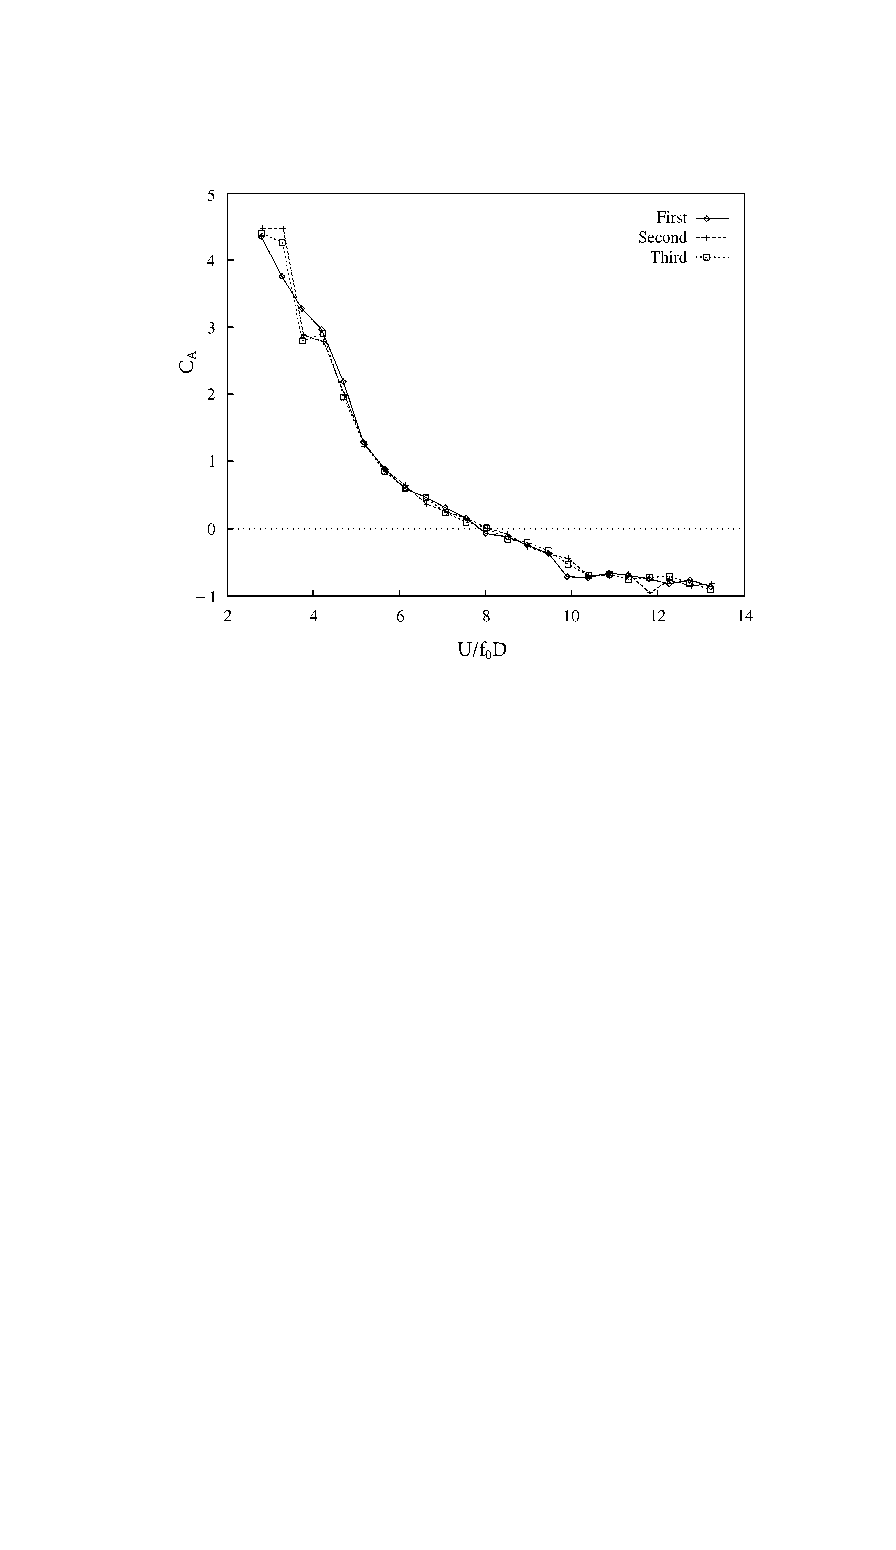
\includegraphics[width=0.7\linewidth]{Figs/caur}
		\caption{Added mass}
		\label{fig:caur}
	\end{subfigure}\\%
	\begin{subfigure}[b]{\linewidth}
		\centering
		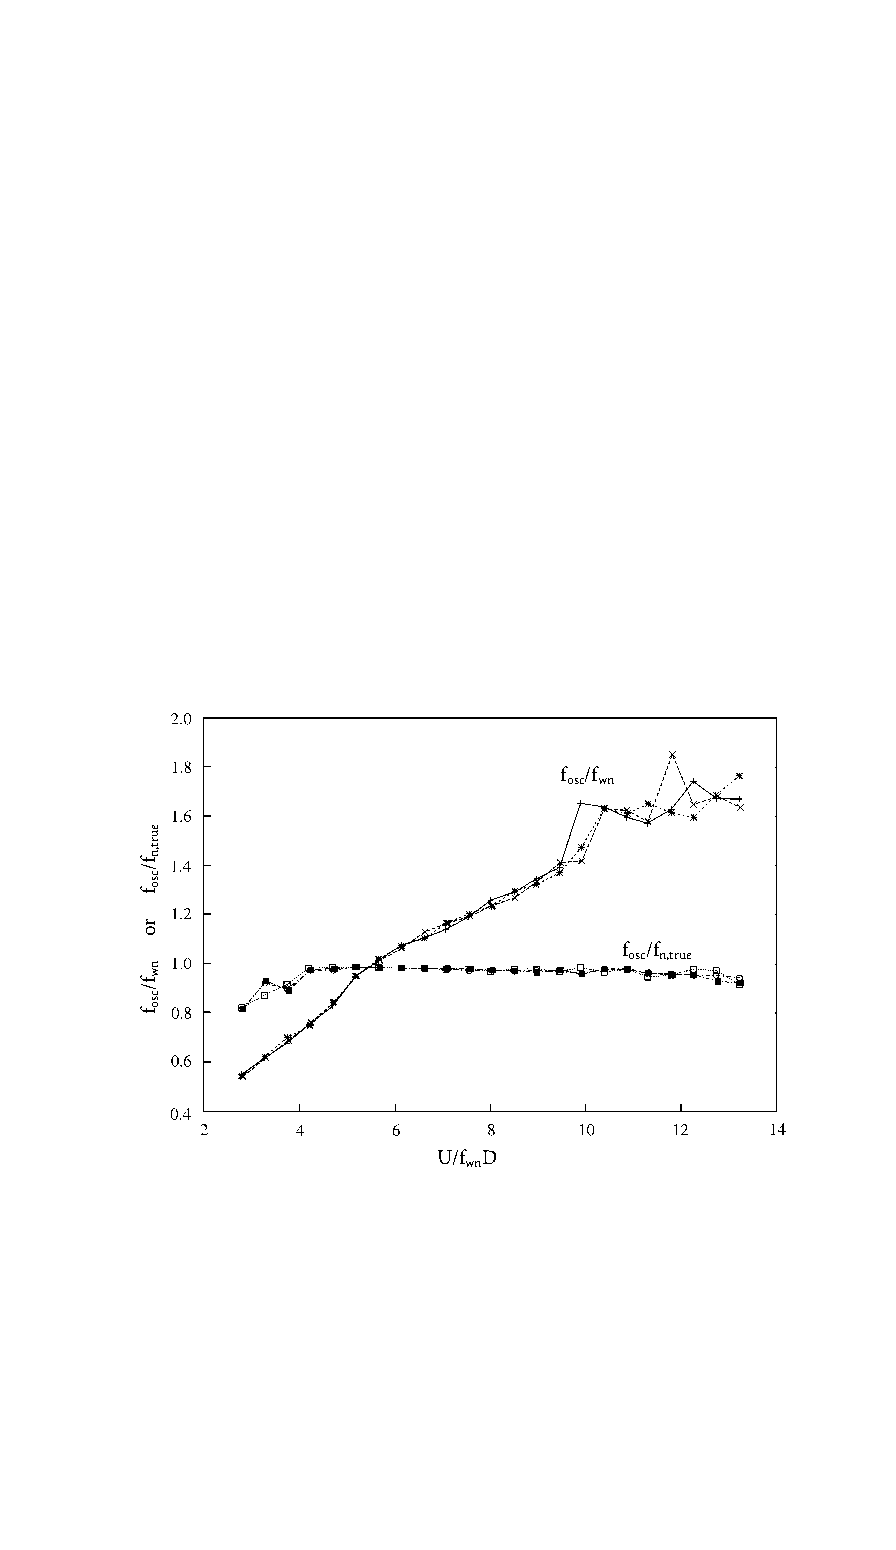
\includegraphics[width=0.7\linewidth]{Figs/fnur}
		\caption{Oscillation frequency}
		\label{fig:fnur}
	\end{subfigure}%
	\caption{
		(a) Added mass and (b) oscillation frequency for VIV of single cylinder in water with $ \mr =1.306$ and $ \dr=0.015 $. (b) shows the mean oscillation frequency divided by natural frequency in still water (0.497 Hz) (sloped lines) and the mean oscillation frequency divided by the true natural frequency using the added mass from Figure 4(a) corresponding to the given reduced velocity (the horizontal lines). \cite{VIKESTAD2000}
	}
	\label{fig:cafnur}
\end{figure}
%$et\,al.$

Vikestad \etal{} \cite{VIKESTAD2000} carried out a series of experiments to measure the true natural frequency $f_n(U_r)$, which was calculated as \Cref{eq:caur,eq:fnur}:
\begin{equation}\label{eq:caur}
C_A=-\frac{8}{nT\rho \pi D^2 L(\omega^2 A)^2} \int_{t}^{t+nT} F \ddot{y} dt
\end{equation}
\begin{equation}\label{eq:fnur}
f_{n,true}(U_r)=\frac{1}{2\pi}\sqrt{\frac{k}{m+\rho V_{cy1} C_A(U_r)}}
\end{equation}
where $ \omega^2 A=\sqrt{2} \ddot{y}_{rms} $, $ nT $ is an integer number $ n $ of oscillation periods $ T $.


%TD: Clearify symbols in these equations

The added mass and mean oscillation as a function of non-dimensional velocity is plotted in \Cref{fig:cafnur} \cite{VIKESTAD2000}. The mean oscillation frequency in \Cref{fig:fnur} was computed as $\sqrt{\ddot{y}_{rms}/y_{rms}}/(2\pi)$. As seen in the figure, the added mass coefficient $ C_A $ drops monotonically with non-dimensional flow speed $ \vr $, causing the true natural frequency $ \fntrue $ to increase as well. 

%CCompare his results with Williamson et al.



%


% 
%what is frequency component?
%sheared #ow
\subsection{Amplitude response types}

\begin{figure}[b!]
	\centering
	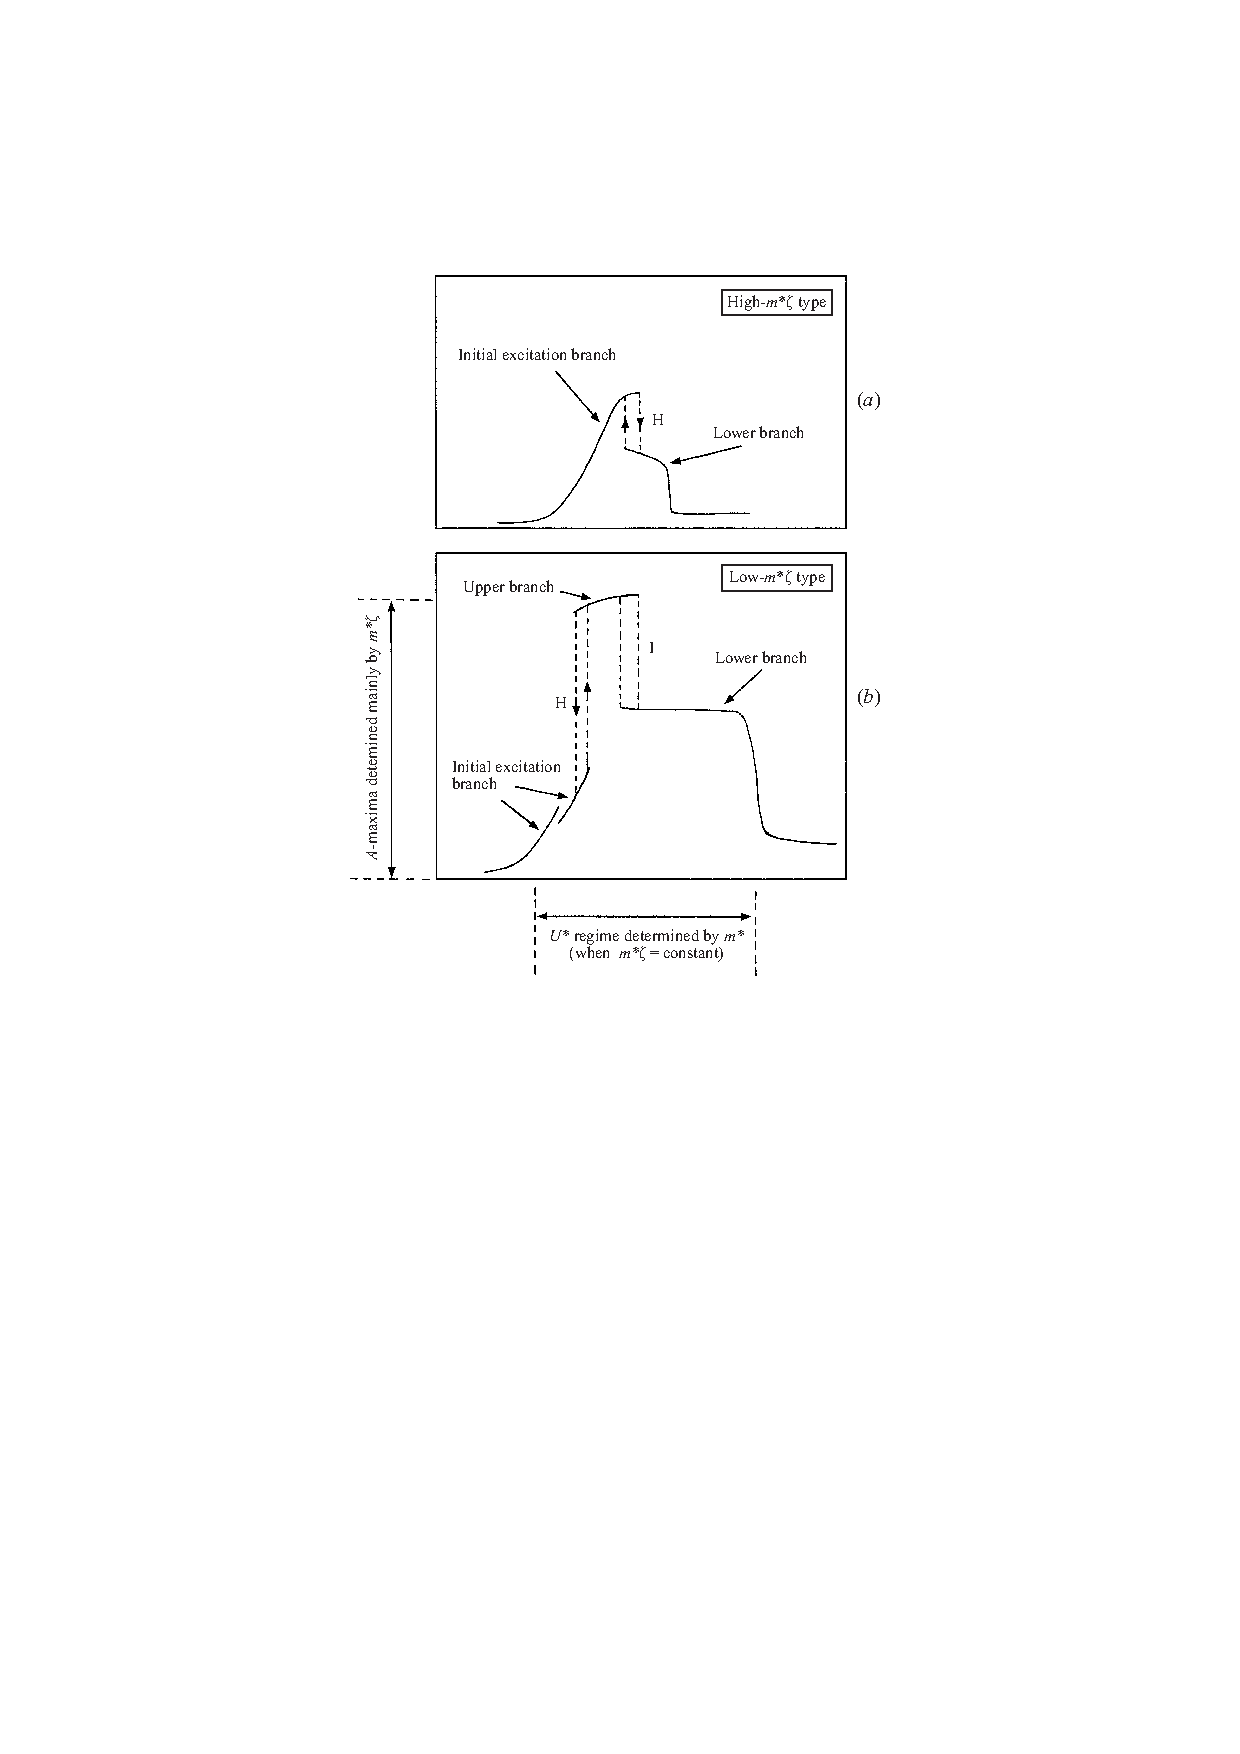
\includegraphics[width=0.55\linewidth]{Figs/tworesponsetypes}
	\caption{The scheme depicts two different types of amplitude response. (Vertical axes represent $A^*$ and horizontal axes represent $U^*$.) The high-(\md{}) type of response discovered by Feng \cite{Feng1968} has two branches (initial and lower), while the low-(\md{}) type of response by Khalak \& Williamson \cite{KHALAK1999} shows three branches (initial, upper and lower). The mode transitions are either hysteretic (H) or involve intermittent switching (I). Khalak \& Williamson stated that the range of synchronization is controlled primarily by $m^*$ (when $m^*\zeta$ is constant), and the peak amplitudes are controlled principally by $m^*\zeta$.}
	\label{fig:tworesponsetypes}
\end{figure}

The response types of an elastically mounted cylinder can be classified into two types by the combined mass-damping parameter (\md{}), as stated by Khalak \& Williamson \cite{KHALAK1999}. Feng \cite{Feng1968} conducted a pioneering experimental study regarding an elastically mounted cylinder with high mass-damping parameter ($m^*\zeta\approx0.25$). Feng found two dissimilar branches regarding amplitude response, which were afterwards termed by Khalak \& Williamson as the "initial branch," where the highest amplitudes are reached, and the "lower branch" (see \Cref{fig:tworesponsetypes}a). Later experiments for a long flexible circular cylinder at high \md{} conducted by Brika \& Laneville \cite{Brika1993} confirmed the existence of the two-branch amplitude response. A hysteresis loop between initial \& lower branches was observed in both experiments (see the "H" in \Cref{fig:tworesponsetypes}a), yet Brika \& Laneville's hysteresis loop (for a long flexible cylinder) was partially different from this illustration. Regarding low $m^*\zeta\approx0.013$, Khalak \& Williamson's experiments \cite{KHALAK1999,Khalak1996,Khalak1997a} identified three branches of response (see \Cref{fig:tworesponsetypes}b). An extra "upper branch" was discovered in addition to the initial \& lower branch. Also, two transitions were identified between these three branches: the hysteretic transition between the initial and upper branches, and the intermittent transition between the upper and lower branches. 
%


The distribution of maximum amplitude $A^*_{max}$ versus the combined mass-damping parameter $(m^*+C_A)\zeta$ (usually called a "Griffin" plot) is demonstrated in \Cref{fig:griffinplot1} \cite{GOVARDHAN2000}, where "Upper" denotes the maximum amplitudes of upper branches, while "Lower" denotes those of the lower branches. A curve line standing for a semi-empirical equation is drawn to compare with some experimental data. The equation aims to represent the vibration of spring-mounted, pivoted or cantilevered cylinders, as well as taut cables, and was compiled originally by Griffin \cite{Griffin1980} in 1980, and then updated by Skop \& Balasubramanian \cite{skop1997new} in 1997. Govardhan \& Williamson reported that, for strictly elastically mounted bluff bodies, some data of $A^*_{max}$ deviate from the curve. This deviation is possibly because the cases with $Re\leq200$ are not considered by the curve, as supported by experimental results from Anagnostopoulos \& Bearman \cite{Anagnostopoulos1992}.

\begin{figure}[tb]
	\centering
	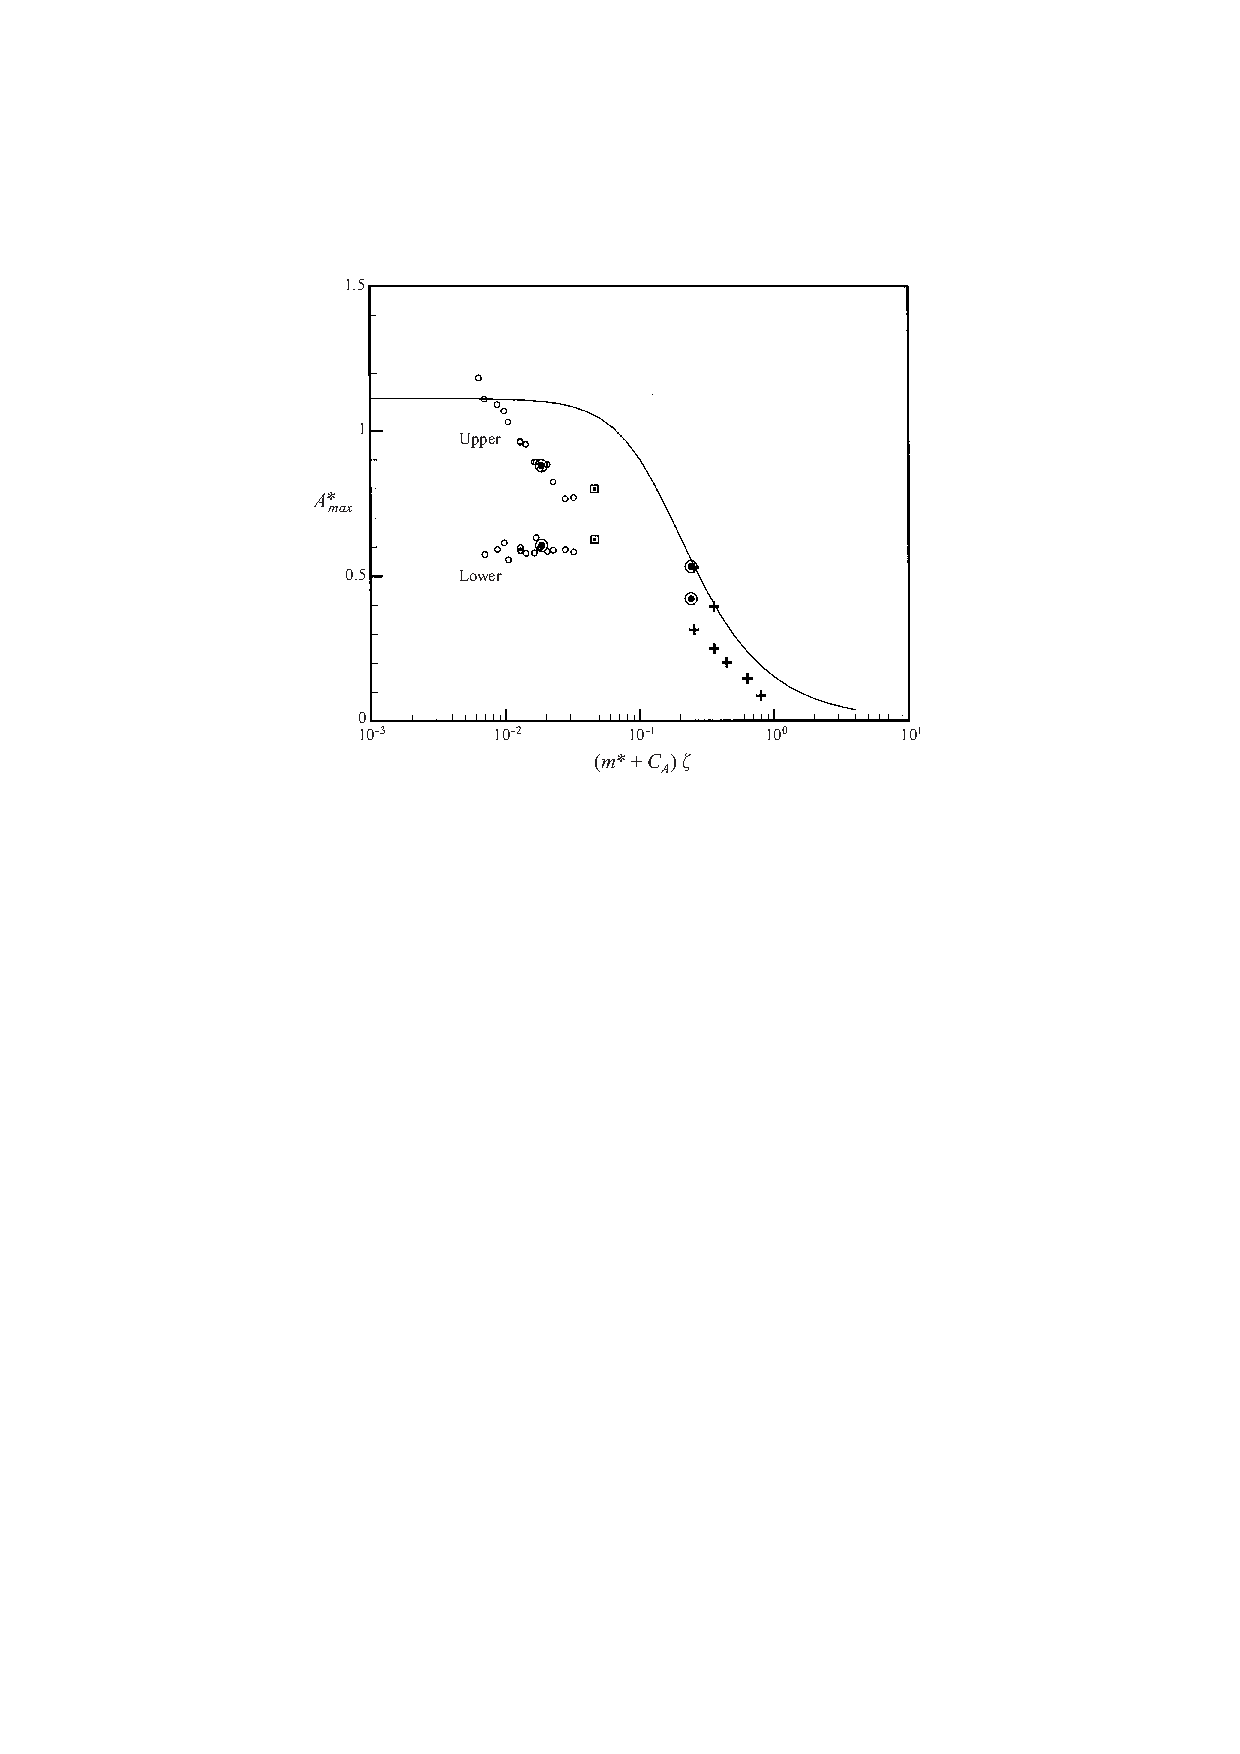
\includegraphics[width=0.7\linewidth]{Figs/griffinplot1}
	\caption{"Griffin" plot by Govardhan \& Williamson \cite{GOVARDHAN2000} shows peak amplitude $A^*_{max}$ versus a combined mass-damping parameter $(m^*+ C_A)\zeta$. Symbols: +, Feng \cite{Feng1968}; $\boxdot$, Hover et al.\cite{Hover1998}; $ \circ $, Khalak \& Williamson \cite{KHALAK1999}; $ \odot $, Govardhan \& Williamson \cite{GOVARDHAN2000};---, Skop \& Balasubramanian \cite{Skop1997}. }
	\label{fig:griffinplot1}
\end{figure}

%Feng \cite{Feng1968} carried out some pioneering experiments for an elastically mounted cylinder under air flow. Feng's results showed that, for high $m^*\zeta$ cases, two amplitude branches are discovered (See Figure ), which were termed as the "initial" and the "lower" branch by Khalak \& Williamson \cite{Khalak1996}. A hysteretic transition is found between branches. Feng's experiments featured very large mass ratio ($m^*\approx250$), as the experiments were conducted in wind tunnel. Many later works focus on smaller mass and damping, and water ($m^*\approx2.5$) was frequently used as the fluid medium.

%Notes:
%? why can we classify R types by the combined mass-damping parameter ???
%Feng, high md:0.25, 0.36(from KW1996, see Parkinson (1989)), Khalak, low md: 0.013, 0.00858,
%check Khalak & Williamson (1996)
%note for Feng, Id=0ma, 100ma, damping current?
%	dimensionless damping coefficient 		   \beta=0.00103, 0.00145
%what is, and why use combined mass-damping parameter $(m^*+C_A)\zeta$ ???
%what is the first "Griffin" plot
%
%\subsection{Added mass}



\subsection{Critical mass ratio}
A critical mass ratio for low mass-damping ratio, (broadly $(m^*+C_A)\zeta < 0.05$), was firstly discovered by Govardhan \& Williamson \cite{GOVARDHAN2000}, who summarised the behaviour of lower branch frequency ($f^*_{lower}=f_{lower}/f_{wn}$) from experimental data from several authors: Govardhan \& Williamson \cite{GOVARDHAN2000}, Hover et al.\@ \cite{Hover1998}, Khalak \& Williamson \cite{KHALAK1999}, and Anand \cite{Torum1985}. By observing the collapse of these experimental data (see \Cref{fig:equation-61}),
\begin{figure}
	\centering
	\captionsetup{justification=centering}
	\includegraphics[width=0.7\linewidth]{"Figs/equation 61"}
	\caption{Distribution of the lower branch frequency (\fslower{}) with x-axis being the mass ratio $m^*$ \cite{GOVARDHAN2000}. The \Cref{eq:61} shows great correspondence with the experimental data from several authors \cite{GOVARDHAN2000,Hover1998, KHALAK1999,Torum1985}, predicting a surge of \fslower{} as $m^*$ decreases towards the critical mass ratio, $m^*_{crit}=0.54$.
	}
	\label{fig:equation-61}
	%figure 20 in GOVARDHAN2000
\end{figure}
\begin{figure}[tbp]
	\centering
	\captionsetup{justification=centering}
	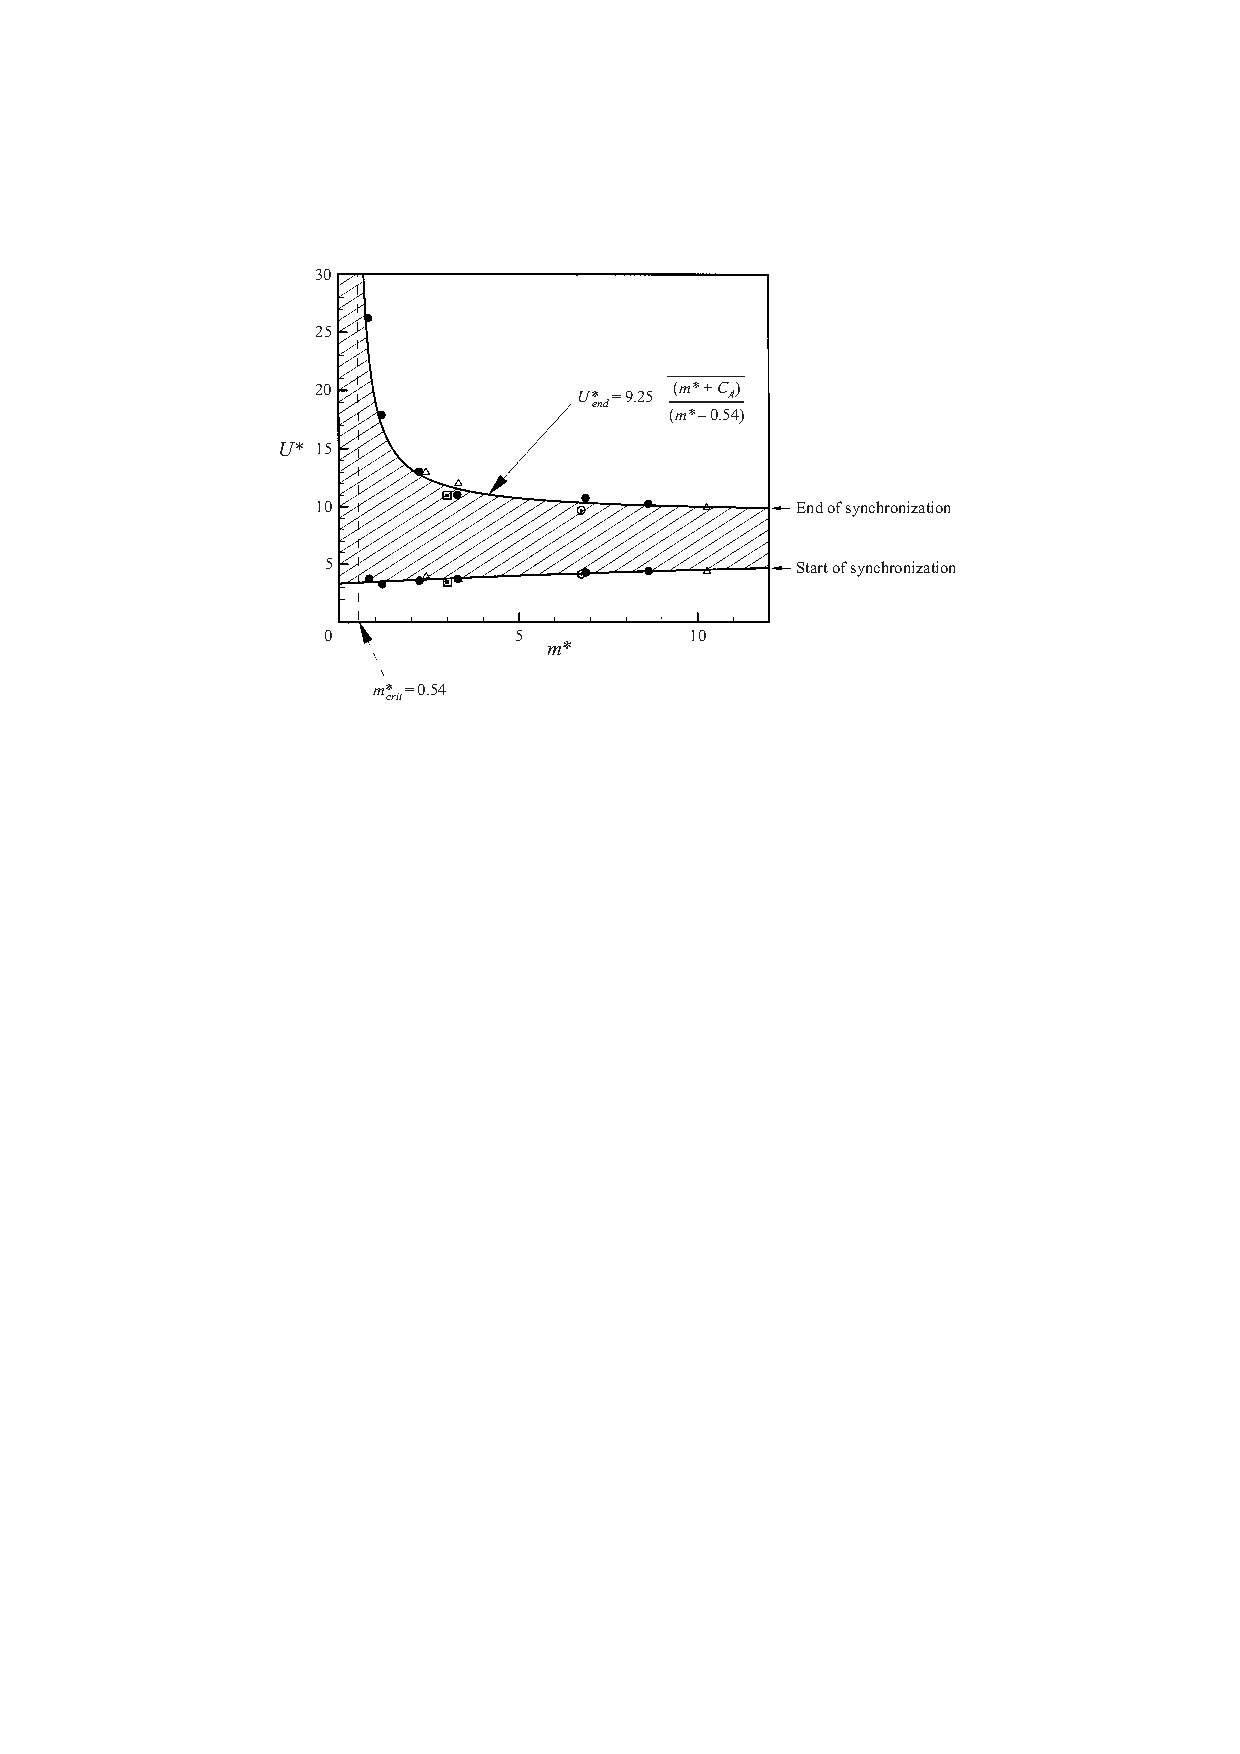
\includegraphics[width=0.8\linewidth]{Figs/syncregime}
	\caption{The shaded area mark the synchronisation regime varying with $m^*$. The equation for \usend{} shows good coherence with the data from several researchers \cite{GOVARDHAN2000,Hover1998, KHALAK1999,Torum1985}. Also, as $m^*$ drops towards $m^*_{crit} = 0.54$, the synchronization regime is greatly extended, and ultimately approaches infinity when $m^*$ drops below $m^*_{crit}$. \cite{GOVARDHAN2000}}
	\label{fig:syncregime}
\end{figure}
Govardhan \& Williamson \cite{GOVARDHAN2000} concluded that if the mass-damping ratio is low, the value of $f^*_{lower}$ depends solely on $m^*$. Moreover, as the cylinder's oscillation syncs with the vortex shedding in lower branch regime, fulfilling the prerequisite of equations \Cref{eq:2,eq:3}, they stated that \Cref{eq:6a} is applicable, and the value of effective added mass ($C_{EA}$) in \Cref{eq:7} depends merely on \{$(U^*/f^*)S, A^*$\}, where $U^*=U/{f_nD}$. The Strouhal number for static cylinder $ S $ is approximately 0.2 because all the experiments mentioned were carried out within the range of $Re \in [200,10^5]$ (see \Cref{fig:strouhalvsre}).
\begin{figure}
	\centering
	%\captionsetup{justification=centering}
	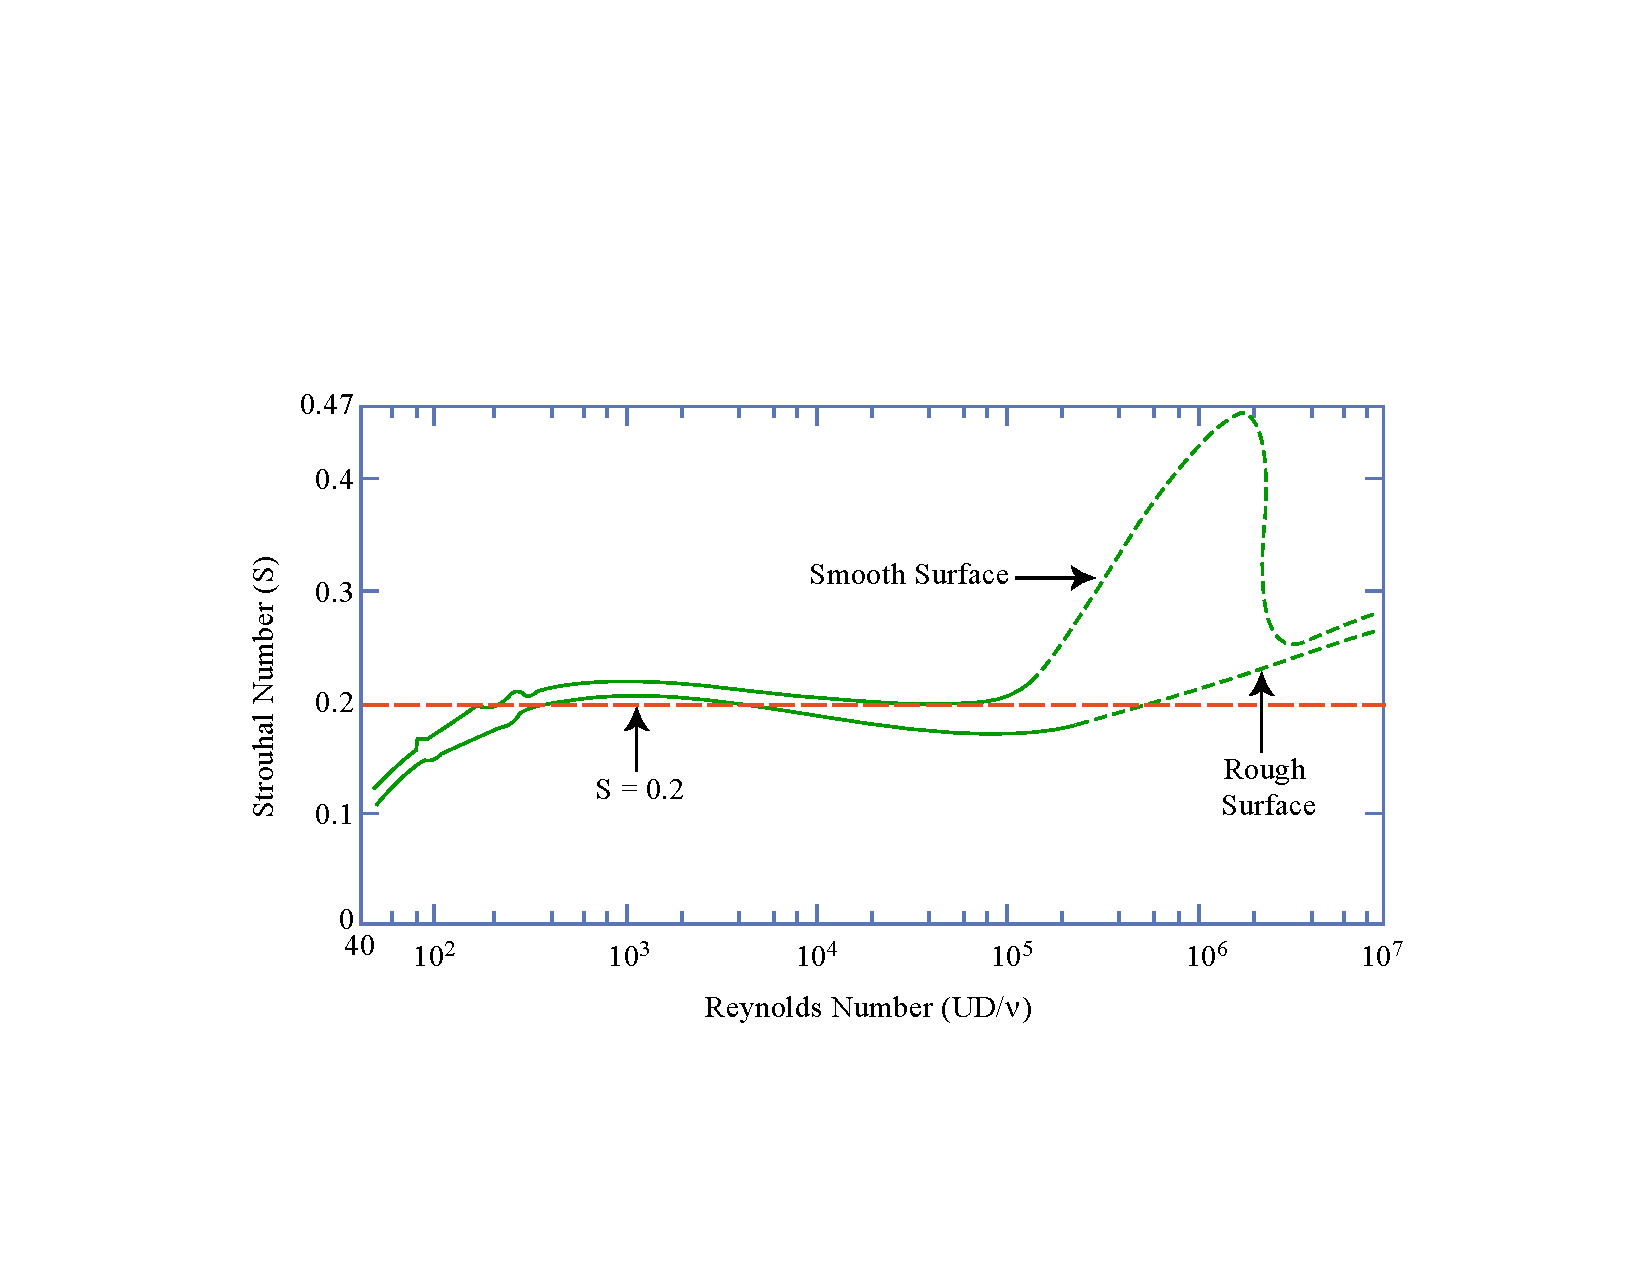
\includegraphics[width=0.9\linewidth]{Figs/StrouhalvsRe}
	\caption{Strouhal number as a function of Reynolds number for circular cylinders. Data from Lienhard \cite{Lienhard1966} and Achenbach and Heinecke \cite{Achenbach2006}. $S\approx0.21 (1-21/Re)$ for $40<Re<200$, from Roshko \cite{roshko1955some}. (plot by Techet \cite{Techet2005} from the VIV lecture note of MIT OCW )}
	\label{fig:strouhalvsre}
\end{figure}
Also, as shown in \Cref{fig:a-vs-ufs},
\begin{figure}
	\centering
	%\captionsetup{justification=centering}
	\includegraphics[width=0.7\linewidth]{"Figs/A vs UfS"}
	\caption{The data of lower branch regimes with two different values of $m^*$ are almost on the same line with the x-axis being $(U^*/f^*)S$, plotted by Khalak \& Williamson \cite{KHALAK1999}. Circular dots: $m^*=1.19$ and $(m^* + C_A)\zeta = 0.0110$; triangular dots: $m^* = 8.63$ and $(m^* + C_A)\zeta = 0.0145$. Solid symbols indicate the lower branch regimes.}
	%figure 17 in GOVARDHAN2000
	\label{fig:a-vs-ufs}
\end{figure}
despite the variation of $m^*$ and $(m^*+C_A)\zeta$, all lower branch data (solid symbols) were plotted along the same line, meaning the variation of $m^*$ does not affect the functional relationship between $(U^*/f^*)S$ and $A^*$, thus not affecting the value of $C_{EA}$. In other words, for lower branch, $C_{EA}$ is a constant in \Cref{eq:6a}.

By fitting experimental data, they found the value of $C_{EA}$ to be $C_{EA}=-0.54\pm0.02$, thus producing \Cref{eq:61}:
\begin{equation}	\label{eq:61}
f^*_{lower}=\frac{f_{lower}}{f_{wn}}=\sqrt{\frac{m^*+C_A}{m^*-0.54}}
\end{equation}
where $C_A=1.0$. \Cref{eq:61} is plotted in \Cref{fig:equation-61}, having good correspondence with the several sets of experimental data. The equation offers a practical prediction to cylinder's lower branch frequency (\fslower{}), provided that the mass ratio ($m^*$) is given, and the mass-damping ratio is low (broadly $(m^*+C_A)\zeta < 0.05$). Also, the critical mass ratio was determined as $m^*_{crit}=0.54$.

\begin{figure}
	\centering
	\captionsetup{justification=centering}
	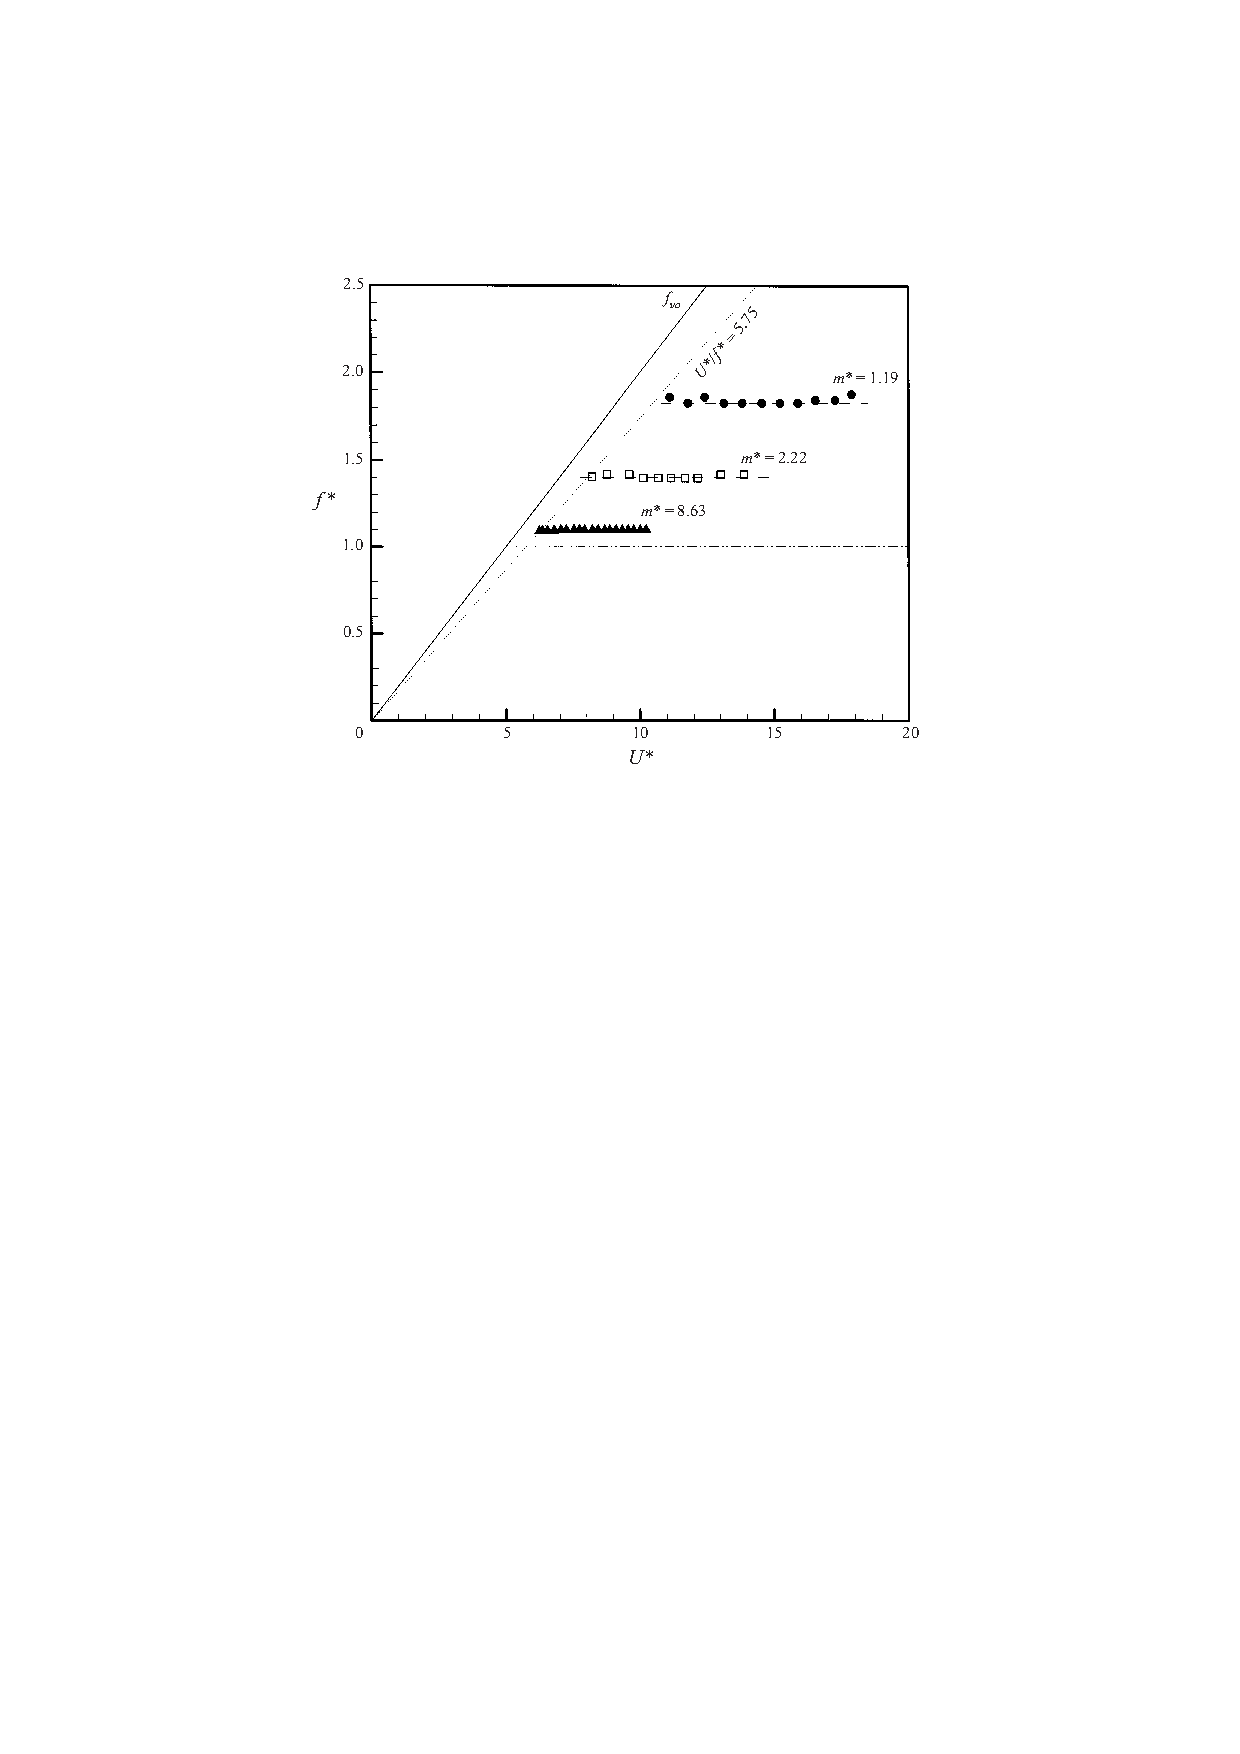
\includegraphics[width=0.7\linewidth]{Figs/ufstart}
	\caption{Lower branch frequency response for low $m^*\zeta$ with different mass ratios, showing a nearly constant value for each specific $m^*$.\cite{GOVARDHAN2000}}
	\label{fig:ufstart}
\end{figure}

In addition, as demonstrated in \Cref{fig:ufstart}, a relationship was summarised from 3 groups of experimental data in \Cref{eq:ufstart}:
\begin{equation}
	U^*_{start}=5.75{f^*_{start}}=5.75f^*_{lower}
	\label{eq:ufstart}
\end{equation}
where the numerical value "5.75" has the experimental accuracy of $\pm0.2$, and $ U^*_{start} $ is the start of the lower branch.

With equations \Cref{eq:61,eq:ufstart}, they \cite{GOVARDHAN2000} further deduced that the start of lower branch regime (regarding reduced flow velocity, $U^*$) can be formulated as \Cref{eq:ulstart}:
\begin{equation}
	U^*_{start} \approx 5.75\sqrt{\frac{m^*+C_A}{m^*-0.54}}
	\label{eq:ulstart}
\end{equation}
From \Cref{eq:ulstart}, it can be seen that $m^* \rightarrow m^*_{crit}$ results in $ U^*_{start} \rightarrow \infty$. They consequently concluded that when mass ratio is below $m^*_{crit}=0.54$, the lower branch will no longer exist, and the synchronisation will not cease with the increase of $U^*$ (see \Cref{fig:syncregime}).

What is more, with similar process, the function to describe the end of lower branch regime --- which is also the end of synchronisation regime --- can be expressed as \Cref{eq:ulend}:
\begin{equation}
U^*_{end} \approx 9.25\sqrt{\frac{m^*+C_A}{m^*-0.54}}
\label{eq:ulend}
\end{equation}

To summarise this section, Govardhan \& Williamson \cite{GOVARDHAN2000} provided an experimentally supported method to predict both the start and the end of the lower branch regime using merely $m^*$, and discovered a critical mass ratio of $m^*=0.54$. However, it is noteworthy that there are two prerequisites for the prediction equations: low mass-damping ratio (broadly $(m^*+C_A)\zeta < 0.05$) and Reynolds number $Re \in [200,10^5]$ (thus $S\approx0.2$). Whether those equations are valid in other conditions appears to remain unchecked. In addition, it is not clearly explained why the effective added mass $C_{EA}$ (see \Cref{eq:7}) is a function of \{$(U^*/f^*)S, A^*$\} (see \Cref{fig:a-vs-ufs}), which is not self-evident, although the final equations match well with the experimental data.


%Notes:
%why C_EA depends merely on \{$(U^*/f^*)S, A^*$\} ?
%why C_A=1? \textbf{comment: why $C_A=1$ ?}
%difference between md and (m+C_A)d
%edit fig. 2.2 U*/f*
%? the starting point of upper branch regime/ start of syncronisation???
% the experiments are under the assumption that S \approx 0.2 for subcritical flow (200<=Re<=10^5)

%\cite{GOVARDHAN2000} \cite{Hover1998} \cite{KHALAK1999} \cite{Torum1985} 
%f_v0 is the vortex shedding frequency in the absence of body oscillations.
%S is the Strouhal number for the static cylinder https://en.wikipedia.org/wiki/Strouhal_number why S=0.2 ??
%S \approx 0.2 for subcritical flow (Re<=10^5)
%initial branch is the 2S mode, and the lower branch is the 2P mode
%
%=====
%
%

%\subsection{Total force $ C_y $ and phase angle $ \phi $}

%The phase angle $ \phi $ between total force $ C_y $ and the displacement $ y $. 



%http://www.annualreviews.org/doi/full/10.1146/annurev.fluid.36.050802.122128
%Feng also noted that the jump in response amplitude was reflected by a significant jump in the phase of the pressure fluctuations relative to body motion. One might suspect that a jump in phase angle (between transverse force and displacement) through resonance, as shown in Figure 2c, will be matched by a switch in the timing of vortex shedding. Zdravkovich \cite{zdravkovich1982modification} showed this for the first time using visualisations from previous studies. An excellent demonstration of this timing switch comes from the comprehensive forced vibration study of Ongoren \& Rockwell \cite{ongoren1988flow}, shown in Figure 3a, where the switch in timing of vortex formation is evident as the body's frequency is increased through a critical value (roughly f/fV ? 1.05). Gu, Chyu \& Rockwell \cite{gu1994timing} confirmed this from forced vibrations at small A* = 0.2, in the groundbreaking first study of this problem using PIV. This phenomenon has also been found in the simulations of Meneghini \& Bearman (1995) \cite{meneghini1995numerical}, Lu \& Dalton (1996) \cite{lu1996calculation}, Blackburn \& Henderson (1999) \cite{blackburn1999study}, Anagnostopoulos (2000) \cite{anagnostopoulos2000numerical} \cite{anagnostopoulos2000numericalb}, Guilmineau \& Queutey (2002) \cite{guilmineau2002numerical}, and further experiments by Krishnamoorthy et al. (2001) \cite{krishnamoorthy2001crosss}.

%\subsection{Vortex-induced vibration in 2-Degree-Of-Freedom}
%Experimental Investigation of Vortex-Induced Vibration in One and Two Dimensions With Variable Mass, Damping, and Reynolds Number




%%\subsection{Lock-in phenomenon}
%
%The lock-in or synchronisation is usually defined as the regime where the oscillation frequency ($f$) and the frequency of vortex formation ($f_V$) approach the natural frequency ($f_{wn}$) of structure, causing large-amplitude vibration. Nevertheless, some studies discovered that large-amplitude vibration also occurs at hundreds of times the natural frequency.
%
%
%
%
%
%%\subsection{High reynolds number}
%
%
%%\subsection{=====}
%
%However,recent studies (inSections2 and 3) show a dramatic departure from this classical result; bodies can conceivably vibrate with large amplitude, at hundreds of times the natural frequency!
%
% The Griffin plot has become an integral part of the offshore design codes (for example, Det Norske Veritas codes), and so it is important to determine it accurately. As discussed in Section 4, a final accurate definition of this important plot is surprisingly not yet available.
% 
% 
% The phenomenon of lock-in, or synchronization (see Blevins 1990, Sumer \& Freds\o{}e 1997), traditionally means that the ratio f* = f/fN remains close to unity, as seen in Figure 2 for high mass ratio. However, for light bodies in water, in this case for $m^*$ = 2.4 in Figure 5, the body oscillates at a distinctly higher frequency (f* = 1.4).
% 
% Therefore, one might define synchronization as the matching of the frequency of the periodic wake vortex mode with the body oscillation frequency. Correspondingly, the force frequency must match the oscillation frequency, which is the definition of lock-in now used by Sarpkaya (1995).
% 
% 
%\textbf{ CA is the potential added mass coefficient (taking the value 1.0)?}
%
% =======
% 
% %\subsection{1 Flow induced vibration of two rigidly coupled circular cylinders in tandem and side-by- side arrangements.pdf}
% 
% the initial branch of the response (where the response amplitude increases with the increasing Vr)
% 
% Definition of branches: see Figure 
%
%
% 
%
%Regarding the frequency response, the classical definition of lock-in or synchronization is often perceived as the regime where the frequency of oscillation (f), as well as the vortex formation frequency (fV), are close to the natural frequency (fN) of the structure throughout the regime of large-amplitude vibration, so that f* = f/fN ? 1 in Figure 2b. 
%
%=====
%
%%\subsection{Numerical Simulation of Vortex-Induced Vibration of Two Rigidly Connected Cylinders in Side-by-Side and Tandem Arrangements Using RANS Model}
%
%Simulations were conducted for a constant mass ratio of 2.5, gap ratios G (ratio of the gap between the cylinders to the cylinder diameter) in the range of 0.5 to 3, and reduced velocities in the range of 1 to 30.
%
%The maximum response amplitude in the lock-in regime was found to occur at G1?40.5 in the side-by-side arrangement, which is about twice that of a single cylinder.
%
%\textbf{ The most fundamental case of flow interaction with multiple cylindrical structures is flow past two circular cylinders close to each other, which has been studied extensively in the past decades.}
%
%The biased flow regime was found when the gap between two side-by-side cylinders was between 0.1D and 1.2D, with D being the diameter of the cylinder, forming a narrow wake behind one cylinder and a wide wake behind another [1,4,6]. Kim and Durbin [5] performed an experimental study on flow past a pair of side-by-side circular cylinders in the subcritical Reynolds number regime and found that the direction of the biased flow changed randomly with time. If two cylinders are in a tandem arrangement in a flow, the vortex shedding from the upstream cylinder was found to be suppressed if the gap between
%1Corresponding author.
%Contributed by the Fluids Engineering Division of ASME for publication in the JOURNAL OF FLUIDS ENGINEERING. Manuscript received November 2, 2014; final manuscript received May 19, 2015; published online September 3, 2015. Assoc. Editor: Francine Battaglia.
%them is less than 2D to 2.5D depending on the Reynolds number [7-9].
%
%ViV of two circular cylinders is not studied as extensively as flow past two stationary cylinders or VIV of a single cylinder. Zdravkovich [10] provided a review of the effects of the interfer- ence between two cylinders on VIV.
%
%Many studies have been con- ducted to study the VIV of an elastically mounted cylinder in the wake of a stationary cylinder. Brika and Laneville [11] and Fon- taine et al. [12] classified the response of two riser pipes in a tan- dem arrangement in two categories: Wake induced oscillation also referred to as galloping and VIV. \textbf{Huera-Huarte and Gharib [13] found that the interference between two cylinders in a side- by-side arrangement was very weak if the center-to-center gap exceeded 3.5 times the cylinder diameter.}
%
%Numerical simulations at low Reynolds numbers have also been conducted to investigate the galloping responses of square cylinders [20,21]. Cui et al. [22] simulated VIV of two elastically connected side-by-side cylinders in a fluid flow and found that the VIV locks onto the first- or the second-mode frequency, depending on the reduced velocity. VIV of two rigidly connected cylinders of different diameters has also been investigated both experimentally [23] and numerically [24] due to their relevance to the piggyback pipeline in offshore engi- neering. It was found that the presence of the small cylinder in the proximity of the large cylinder had significant effects on the vor- tex shedding regime and vibration amplitude of the large cylinder.
%
%In the offshore oil and gas industry, a bundle of pipelines or riser pipes are often strapped together due to economical and operational considerations.
%
%modify it for my version [In this study, VIV of two identical rigidly con- nected cylinders in side-by-side and tandem arrangements is investigated numerically by solving the 2D RANS equations. The aim of the study is to identify the effects of the distance between the two cylinders on the vibration amplitude of the cylinder sys- tem in both arrangements through extensive numerical simula- tions. The mechanisms of the VIV and the flow patterns that are correlated to VIV are discussed in detail. Simulations are con- ducted for one degree-of-freedom VIV in the cross-flow direction of two rigidly connected cylinders for gap ratios (gap to diameter ratio) ranging from 0.5 to 3 with an increment of 0.5 and reduced velocities ranging from 2 to 30 with an increment of 0.5.] 
%
%justification of the 2D RANS model k-omega, double check the code, see if the models are the same [ The shear stress transport (SST) k-x model [25] is used to close the RANS equation. The SST k-x model provides a good prediction of flows involving adverse pressure gradient and has the ability to accurately predict pressure-induced separation [25]. The validation of the RANS equation with k-x model in the simu- lation of VIV has been demonstrated in a number of previous studies [26,27]. \textbf{CHECK: Zhao et al. [28] also demonstrated that the two- dimensional RANS model improves the VIV solution significantly compared with the 2D Navier?Stokes equations.} ]
%
%The RANS equations and the SST k-x equations are solved using the Petrov?Galerkin FEM developed by Zhao et al. [29].
%
%Validation:
%
%Zhao [31] validated the numerical model in the simulation of flow past two side-by-side stationary cylinders and obtained good agreement between the numerical results and the experimen- tal data in Ref. [6]. Zhao and Cheng [26] validated the numerical model used in this study by comparing the numerical results with the experimental data of two degrees-of-freedom vibration of a circular cylinder at $m^*$ 1?4 2.4, f 1?4 0.000575, and Re 1?4 1000 to 15000 (corresponding to Vr 1?4 1?15) in Ref. [32]. Cui et al. [22] validated the present numerical model by comparing the numerical results of flow-induced vibration of the downstream cylinder of two cylinders in a tandem arrangement with the experimental data in Ref. [33]. The numerical results in these validation works were found to agree well with the experimental data. Since the nu- merical model in this study has been validated in previous studies, the validation is not repeated.
%
%get the constants in k-omega model: make a table of \textbf{7 parameters}
%
%read more! 
%[1] Zdravkovich, M. M., 1977, ?Review of Flow Interference Between Two Circu- lar Cylinders in Various Arrangements,? ASME J. Fluids Eng., 99(4), pp. 618?633.
%[2] Zdravkovich, M. M., 1987, ?The Effects of Interference Between Circular Cylinders in Cross Flow,? J. Fluids Struct., 1(2), pp. 239?261.
%[3] Sumner, D., 2010, ?Two Circular Cylinders in Cross-Flow: A Review,? J. Fluids Struct., 26(6), pp. 849?899.
%[10] Zdravkovich, M. M., 1988, ?Review of Interference-Induced Oscillations in Flow Past Two Parallel Circular Cylinders in Various Arrangements,? J. Wind Eng. Ind. Aerodyn., 28(1?3), pp. 183?200.
%[28] Zhao, M., Cheng, L., An, H., and Lu, L., 2014, ?Three-Dimensional Numerical Simulation of Vortex-Induced Vibration of an Elastically Mounted Rigid Circu- lar Cylinder in Steady Current,? J. Fluids Struct., 50, pp. 292?311.
%[29] Zhao, M., Cheng, L., Teng, B., and Dong, G., 2007, ?Hydrodynamic Forces on Dual Cylinders of Different Diameters in Steady Flow,? J. Fluids Struct., 23(1), pp. 59?83.
%[32] Jauvtis, N., and Williamson, C. H. K., 2004, ?The Effect of Two Degrees-of- Freedom on Vortex-Induced Vibration at Low Mass and Damping,? J. Fluid Mech., 509, pp. 23?62.
%
%======
%%\subsection{MIT VIV lecture note}
%
%
%classical one cylinder under external steady flow:
%
%Due to the alternating vortex wake (?Karman street?) the
%oscillations in lift force occur at the vortex shedding frequency
%and oscillations in drag force occur at twice the vortex
%shedding frequency.
%
%\begin{figure}[h]
%	\begin{center}
%		\quad
%		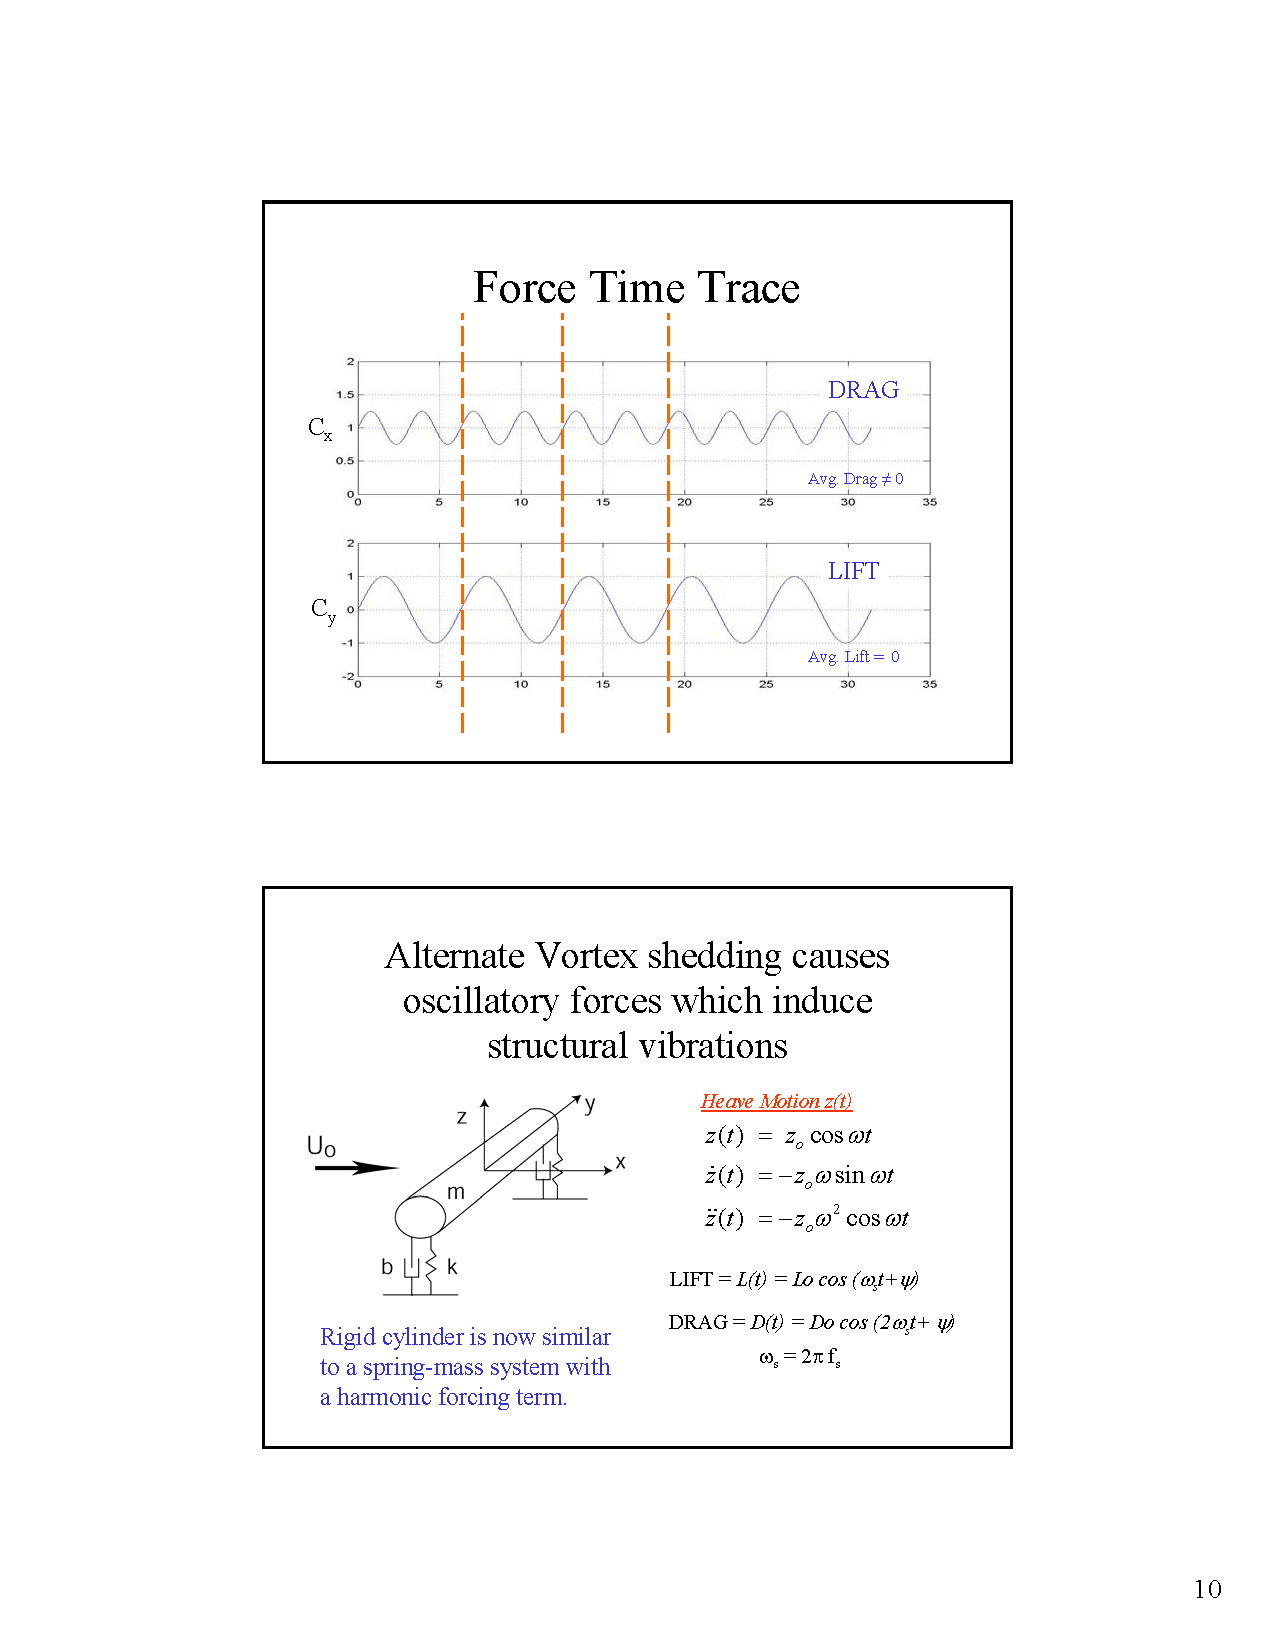
\includegraphics[width=0.5\textwidth]{./Figs/MIT-VIV-lecture-note-page10.pdf}
%	\end{center}
%\end{figure}
%\begin{figure}[h]
%	\begin{center}
%		\quad
%		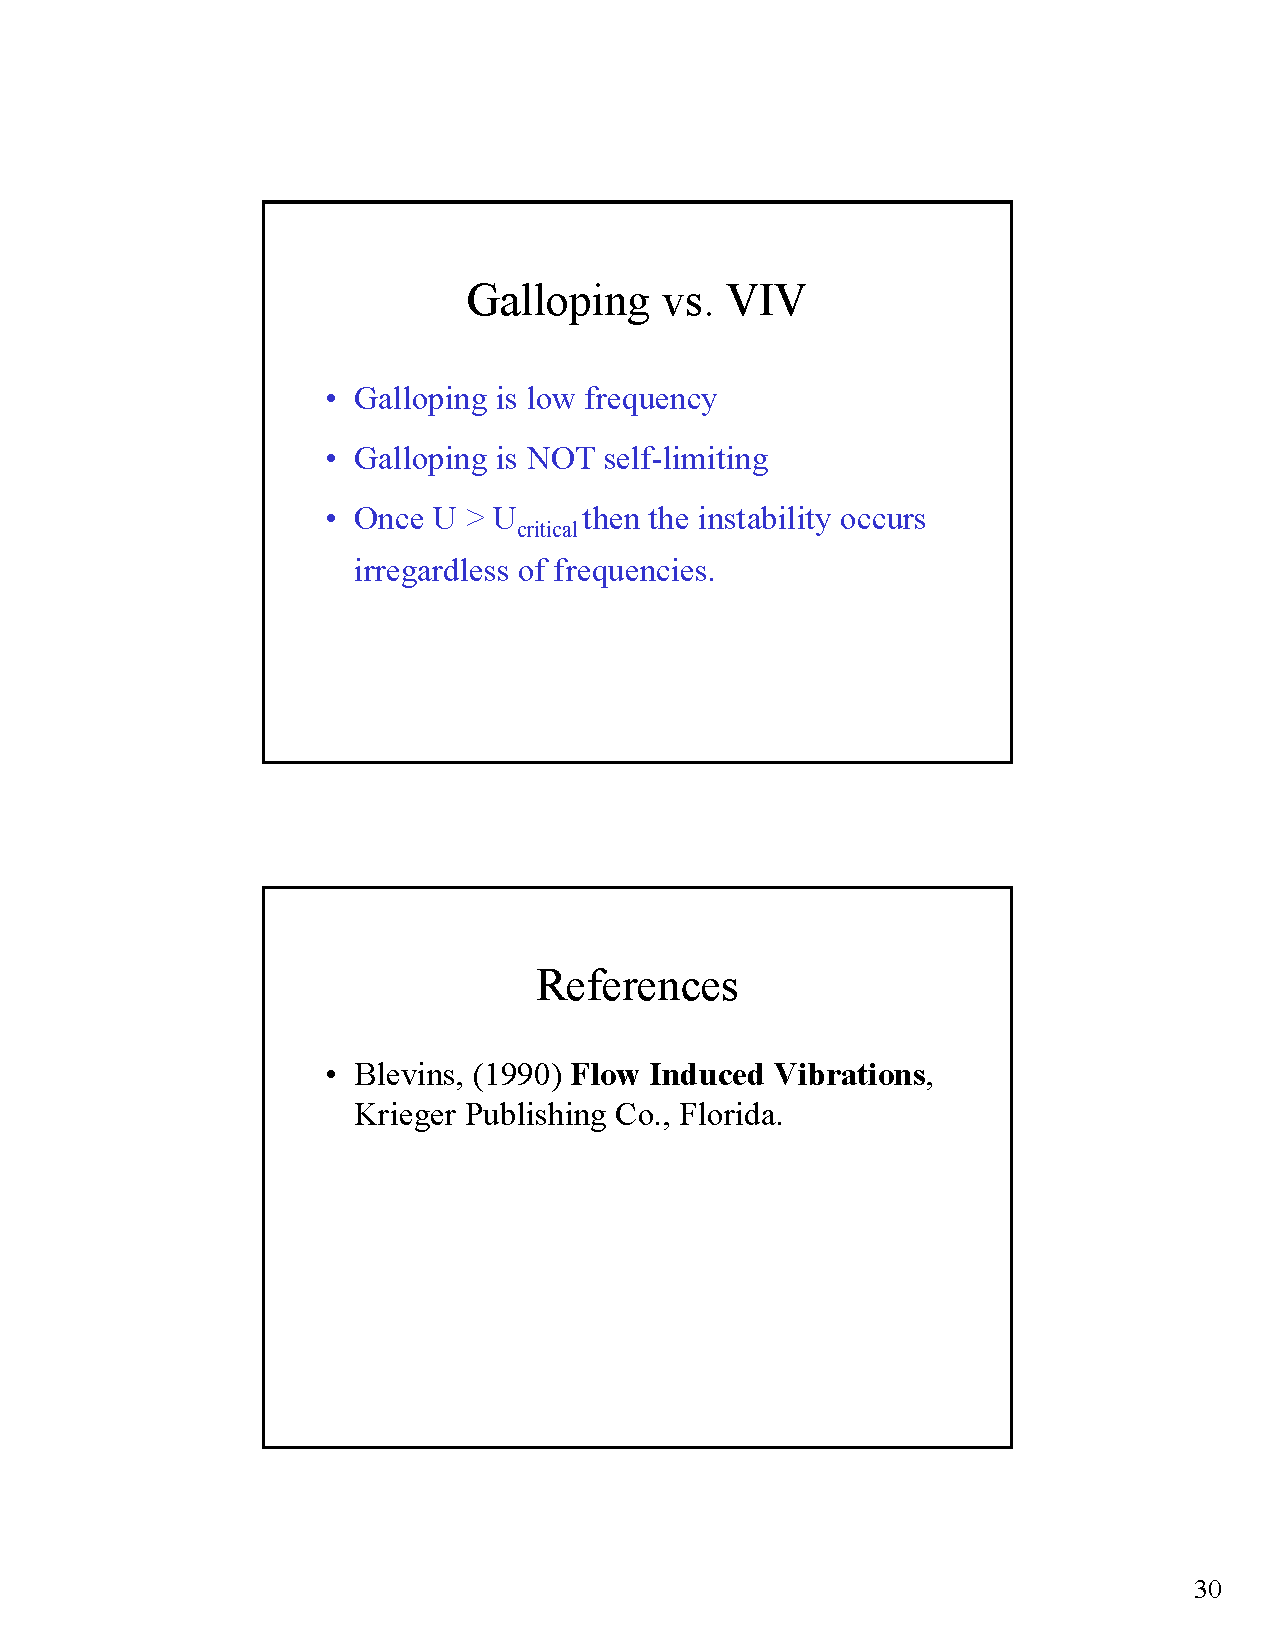
\includegraphics[width=0.5\textwidth]{./Figs/MIT-VIV-lecture-note-p30-galloping.pdf}
%	\end{center}
%\end{figure}
%
%high mass ratio, $m^*$~250 >>1. 
%
%====
%
%%\subsection{Oxford VIV group: http://www.eng.ox.ac.uk/tidal/research/viv-cylinder}
%
%A fluid flow past a bluff body, such as a circular cylinder, will result in the periodic shedding of vortices into the body?s wake for all but the lowest flow speeds. This process gives rise to oscillatory lift and drag forces which, if the body is compliant or elastically supported, can result in Vortex-Induced Vibrations (VIV). VIV can in turn lead to fatigue damage in vibrating structures, which makes it an important issue in the design of bridges, chimney stacks and marine riser pipes.
%
%The principal aim of the low Reynolds number VIV research is to use numerical models to further the understanding of the types of synchronisation that can exist between the vortex shedding form a cylinder submerged in a flow and the motion of the cylinder. A high order spectral element Computational Fluid Dynamics (CFD) code, Nektar, is employed to compute fluid flow past a circular cylinder that is undergoing vibrations transverse to the direction of the flow. Presently the mode of vortex shedding, which describes the manner in which the vortices are formed at the surface of the cylinder and is an indicator of the level of synchronisation that exists between the cylinder and the shedding, has been carefully analysed over a wide parameter space and has exposed some interesting trends. \textbf{The lift component of the lift force acting in-phase with the cylinder's velocity contains information relating to the direction of power transfer between the fluid and cylinder: whether the fluid is exciting or damping the motion of the cylinder}; the present research has shown good agreement with experimental data in this respect, and has uncovered the hitherto unknown reason for which hysteretic responses are often observed in laboratory experiments.
%
%Fatigue damage due to VIV in marine riser pipes represents a significant problem for the offshore oil industry. Current industry-standard VIV prediction strategies involve the use of very large safety factors, which is unsatisfactory from an engineering perspective. A means by which VIV response can be accurately and reliably predicted is therefore extremely desirable. The work of the group in this area focuses on the use of a two ?dimensional CFD code, VIVIC, to predict such riser pipe vibrations. The code takes a [strip theory approach], whereby fluid flow is computed on multiple two-dimensional planes that are positioned at intervals along the axis of a long vibrating pipe, modelled by a Finite Element assemblage. The model permits motions in both the in-line, x, and cross-flow, y, directions. By numerically simulating the experimental set-up of Trim et al (Journal of Fluids and Structures, 2005), the research has shown that VIVIC is capable of accurate simulation of in-line and cross-flow VIV, and has indicated that travelling waves are predominant along the length of the pipe, even when the flow profile is uniform. Super-harmonic responses have been also been observed, and they have been shown to be dominant with respect to riser curvature in a number of instances. Furthermore, [fatigue analysis] has revealed that the super-harmonic responses cab increase fatigue damage rate by an order of magnitude in the in-line direction and by two orders in the cross-flow direction.
%
%====
%
%%\subsection{MOTIONS, FORCES AND MODE TRANSITIONS IN VORTEX-INDUCED VIBRATIONS AT LOW MASS-DAMPING 1999}
%\label{section MOTIONS, FORCES AND MODE TRANSITIONS}
%These experiments, involving the transverse oscillations of an elastically mounted rigid cylinder at very low mass and damping, have shown that there exist two distinct types of response in such systems, depending on whether one has a low combined mass-damping parameter (low $m^*$?), or a high mass-damping (high$m^*$? ). For our low $m^*$?, we find three modes of response, which are denoted as an initial amplitude branch, an upper branch and a lower branch. For the classical Feng-type response, at high$m^*$? , there exist only two response branches, namely the initial and lower branches. The peak amplitude of these vibrating systems is principally dependent on the mass-damping ($m^*$?), whereas the regime of synchronization (measured by the range of velocity U*) is dependent primarily on the mass ratio, $m^*$?. At low ($m^*$?), the transition between initial and upper response branches involves a hysteresis, which contrasts with the intermittent switching of modes found, using the Hilbert transform, for the transition between upper?lower branches. 
% 
%\textbf{ A 180 degrees jump in phase angle ? is found only when the flow jumps between the upper-lower branches of response.}
%
%The good collapse of peak-amplitude data, over a wide range of mass ratios ($m^*$=1?20), when plotted against ($m^*$+CA) ? in the "Griffin" plot, demonstrates that the use of a combined parameter is valid down to at least ($m^*$+CA)? ~0.006. This is two orders of magnitude below the ?limit? that had previously been stipulated in the literature, ($m^*$+CA) ?>0.4. 
%
%\textbf{Using the actual oscillating frequency (f) rather than the still-water natural frequency (fN), to form a normalized velocity (U*/f*), also called "true" reduced velocity in recent studies}, we find an excellent collapse of data for a set of response amplitude plots, over a wide range of mass ratios $m^*$ . Such a collapse of response plots cannot be predicted a priori, and appears to be the first time such a collapse of data sets has been made in free vibration. The response branches match very well the Williamson-Roshko (Williamson \& Roshko 1988) map of vortex wake patterns from forced vibration studies. Visualization of the modes indicates that the initial branch is associated with the 2S mode of vortex formation, while the Lower branch corresponds with the 2P mode. Simultaneous measurements of lift and drag have been made with the displacement, and show a large amplification of maximum, mean and fluctuating forces on the body, which is not unexpected. It is possible to simply estimate the lift force and phase using the displacement amplitude and frequency. This approach is reasonable only for very low $m^*$.
%
%In the relatively simple case of the elastically mounted cylinder there exist, however, some fundamental questions concerning vibration phenomena for very low mass and damping, for which there are very few laboratory investigations. (note: \textbf{at 1999})
%
%\textbf{ Q2: Modes of VIV for 1 cylinder}
%
%\textbf{ Q3: usefully define synchronisation or lock-in}
%
%Bearman (1984), for example, discusses in his review that for large mass ratios ($m^*$>>1), the actual cylinder oscillation frequency ( $f$ ) at resonance will be close to the vortex-shedding frequency for the static cylinder ( $f_O$  ), and also close to the system natural frequency ($f_{wn}$), i.e.\ $f \approx f_O \approx f_N$.
%
%
%
%Despite the extensive use of the log-log "Griffin" plot by practicing engineers (it is included for example in the standard codes of Det Norske Veritas), it is not known precisely under what conditions the assumptions regarding (U*/f*) and f* would hold, that would lead to a "unique'' curve of $A^*_{max}$    versus S7. Problems regarding the validity of this widely used plot were pointed out clearly by Sarpkaya (1978, 1979) and by Bearman (1984), and others. Bearman states that, in the case of small $m^*$, even if $m^*\zeta$ , or equivalently $(m^*+C_A)\zeta$, is kept constant, the frequency f * will be affected by independent variations of mass ratio $m^*$, as evident from our equation (5). Therefore, one might expect that the peak response $A^*_{max}$    will not be a unique function of the combined $m^*\zeta$  parameter. However, the effects of individual variation of $m^*$, for example, might be negligibly small, under some circumstances. This raises the important question, which we shall address in the present paper: What range of values of $m^*$ and $\zeta$ will yield, to good accuracy, a single relation between $A^*_{max}$    and $m^*\zeta$?
%
%========
%
%In the offshore oil and gas industry, a bundle of pipelines or riser pipes are often strapped together due to economical and operational considerations.
%
%========
%
%%********************************** %Second Section  *************************************
%%\section{Natural frequency} %Section - 1.2
%%\label{section1.2}
%Added mass coefficient $C_A$?
%
%=====
%
%Wikipedia:  https://en.wikipedia.org/wiki/Resonance
%
%
%\textbf{Some systems have multiple, distinct, resonant frequencies.}
%
%In physics, resonance describes when a vibrating system or external force drives another system to oscillate with greater amplitude at a specific preferential frequency.
%
%Increase of amplitude as damping decreases and frequency approaches resonant frequency of a driven damped simple harmonic oscillator.[1][2]
%
%Frequencies at which the response amplitude is a relative maximum are known as the system's resonant frequencies or resonance frequencies. At resonant frequencies, small periodic driving forces have the ability to produce large amplitude oscillations. This is because the system stores vibrational energy.
%
%Resonance occurs when a system is able to store and easily transfer energy between two or more different storage modes (such as kinetic energy and potential energy in the case of a pendulum). However, there are some losses from cycle to cycle, called damping. When damping is small, the resonant frequency is approximately equal to the natural frequency of the system, which is a frequency of unforced vibrations. Some systems have multiple, distinct, resonant frequencies.
%
%Mechanical resonance is the tendency of a mechanical system to absorb more energy when the frequency of its oscillations matches the system's natural frequency of vibration than it does at other frequencies. It may cause violent swaying motions and even catastrophic failure in improperly constructed structures including bridges, buildings, trains, and aircraft. When designing objects, engineers must ensure the mechanical resonance frequencies of the component parts do not match driving vibrational frequencies of motors or other oscillating parts, a phenomenon known as resonance disaster.



\section{Flow around Two Cylinders}  \label{sec:fa2} %Section - 1.3 
%\label{section1.3}
%TD: include time histories in the Result chapter
%1DOF, Re=5000, m*=2.5, G=gap/D=0.5~3.0, Vr=1~30, Numerical Simulation of Vortex-Induced Vibration of Two Rigidly Connected Cylinders in Side-by-Side and Tandem Arrangements Using RANS Model, 
%1DOF, Re=150, m*=2.0, G=(centre2centre distance)/D=1.5, 2, 4, 6, Vr= 0.5:0.5:15 for tandem, Vr= 0.5:0.5:30 for side-by-side.    Flow induced vibration of two rigidly coupled circular cylinders in tandem and side-by-side arrangements at a low Reynolds number of 150
%
Two closely placed stationary circular cylinders with identical diameters exposed to flow are the most basic case for flow interaction with multiple cylindrical structures, which has been studied extensively in the past decades \cite{Zdravkovich1977b,Zdravkovich1987a,Sumner2010}. This section reviews previous studies for both two stationary \& elastically mounted cylinders.

The most common configurations for two stationary cylinders are the side-by-side arrangement and tandem arrangement. For two cylinders in the side-by-side arrangement, it was found that the gap between the cylinders is an important factor for the flow pattern. If the gap between two cylinders is small, they behave as a single bluff body followed by a single wake \cite{Williamson1985a,Kim1988}. While the gap between cylinders is from $ 0.1D $ to $ 1.2D $ ($ D $ is the diameter of each cylinder), the biased flow occurs for certain experimental conditions and the Reynolds number, producing a wide wake behind one cylinder and a narrow wake behind another \cite{Zdravkovich1977b,Williamson1985a,alam2003aerodynamic}. In the subcritical Reynolds number regime, the direction of the biased flow changes randomly with time. For two cylinders in tandem arrangement, if the gap is less than $ 2D $ to $ 2.5D $ depending on the Reynolds number, the vortex shedding from the upstream cylinder is suppressed \cite{tasaka2006hysteretic,Mizushima2005,Meneghini2001}. 

%WHat is gallpoping? flow interference?

 In terms of VIV for elastically mounted cylinders, studies were carried out for stationary cylinder and a downstream flexible cylinder, and it was found that responses of two riser pipes are categorised into two types: wake induced oscillation (i.e.\ galloping) and VIV \cite{Brika1999, fontaine2005riser}. Furthermore, for two cylinders (both elastically mounted) in a side-by-side arrangement, the interference between them is very weak if the centre-to-centre distance surpasses 3.5 times the cylinder diameter \cite{Huera-Huarte2011}. In terms of numerical studies, VIV of two cylinders in tandem were mainly simulated at relatively low Reynolds numbers ($Re \leq1000$) \cite{anagnostopoulos1998numerical,Mittal1999,Mittal2001,Mittal*2004,jester2004numerical,Sen2011}. Numerical simulations for the galloping responses of square cylinders also focused on low Reynolds numbers \cite{Sen2011,Joly2012}. For VIV of two rigidly connected cylinders with different diameters, experimental \cite{Zang2014} and numerical \cite{Rahmanian2014} studies have been carried out motivated by the piggyback pipeline in offshore engineering, and the small cylinder in the proximity of the large cylinder was found to have great impact on the oscillation and vortex wake of the large cylinder.
 
 %Galloping is driven by a time-averaged fluid force which develops in phase with the structural velocity and has a frequency many times lower than the vortex shedding frequency. \cite{Robertson2003}
 
 Another classic configuration for VIV study is two identical rigidly connected cylinders with 1DOF, which is to investigate a bundle of pipelines or risers subjected to flows in natural environment. Considering the numerical simulation at low Reynolds number ($ Re=150 $), low mass ratio ($ m^*=2.0 $), and no damping ($ \zeta=0 $)\cite{Zhao2014b}, for side-by-side arrangement, a combination of VIV and galloping is found to occur at $ L/D = 1.5 $ and 2. For tandem arrangement, the critical gap for the onset of vortex shedding from the upstream cylinder is significantly less than that for two stationary cylinders, while the critical gap is slightly greater than that at high Reynolds numbers. 
 
 In terms of high Reynolds number ($ Re=5000 $), low mass ratio ($ m^*=2.5 $), no damping ($ \zeta=0 $) using RANS model \cite{zhao2016numerical}, for side-by-side arrangement, the maximum response amplitude was found to occur at $ G=0.5 $, which is roughly twice the amplitude for that of the single cylinder VIV. It is interesting that for $ G=1.5 $, 2, 2.5, and 3, the response amplitude was reported to be zero as the reduced velocity goes beyond 7, 6, 6, and 6.5, respectively, as the vortex shedding for each of two cylinders are out of phase with each other. For the tandem arrangement, the response amplitude for two cylinders is larger than that of a single cylinder for $ G= 0.5\sim2.5$. In addition, the phenomenon of asymmetric vortex shedding is observed as seen in \Cref{fig:2casymetricpat}.


\begin{figure}[tbp]
\centering
	\captionsetup{justification=centering}
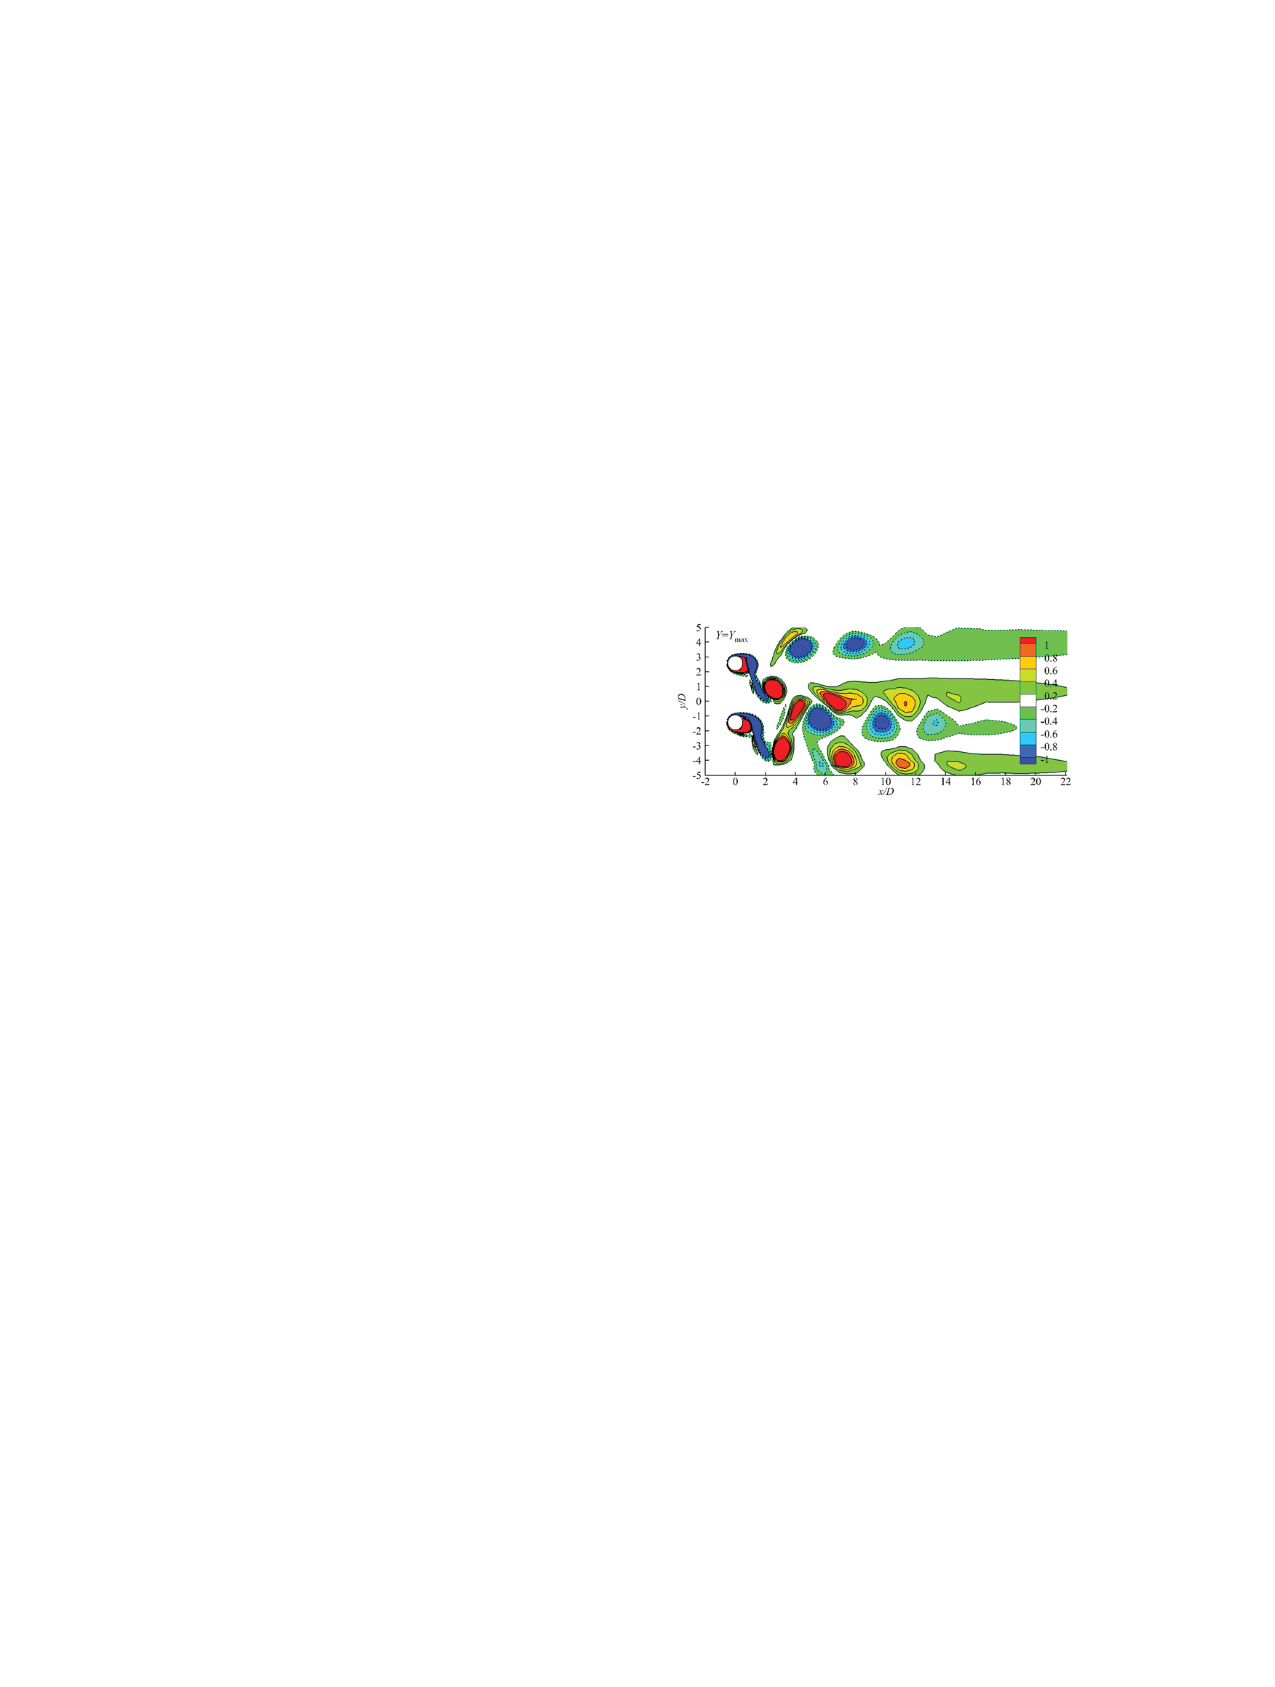
\includegraphics[width=0.7\linewidth]{Figs/2casymetricpat}
\caption{Vorticity contours for two elastically mounted and rigidly connected cylinders in the side-by-side arrangement at $ G=3,\ V_r=5,\ Re=5000,\ m^*=2.5,\ \zeta=0 $. \cite{zhao2016numerical}}
\label{fig:2casymetricpat}
\end{figure}

%====

In summary of this section, it can be seen that, despite useful conclusions found and interesting phenomena discovered, only a limited number of experimental or numerical studies were carried out regarding the investigation of two-cylinder cases, especially the elastically mounted and rigidly connected two cylinders in high Reynolds condition, where quantitative relationships between the inputted experimental configurations (e.g.\ gap ratio) and the outputted simulation results (e.g.\ vorticity contours) have not already been constructed. In addition, all the two-cylinder cases reviewed are exposed to moving fluid - none in still water, so there is clearly a need for more research in this area. See \Cref{cha: numerical results} for more details of what I have done.

\section{Flow around Cylinder Arrays} \label{sec:fa>2}
%cite: FLOW-INDUCED VIBRATIONS IN ARRAYS OF CYLINDERS

\begin{figure}[tbp]
	%\captionsetup{justification=centering}
	\centering
	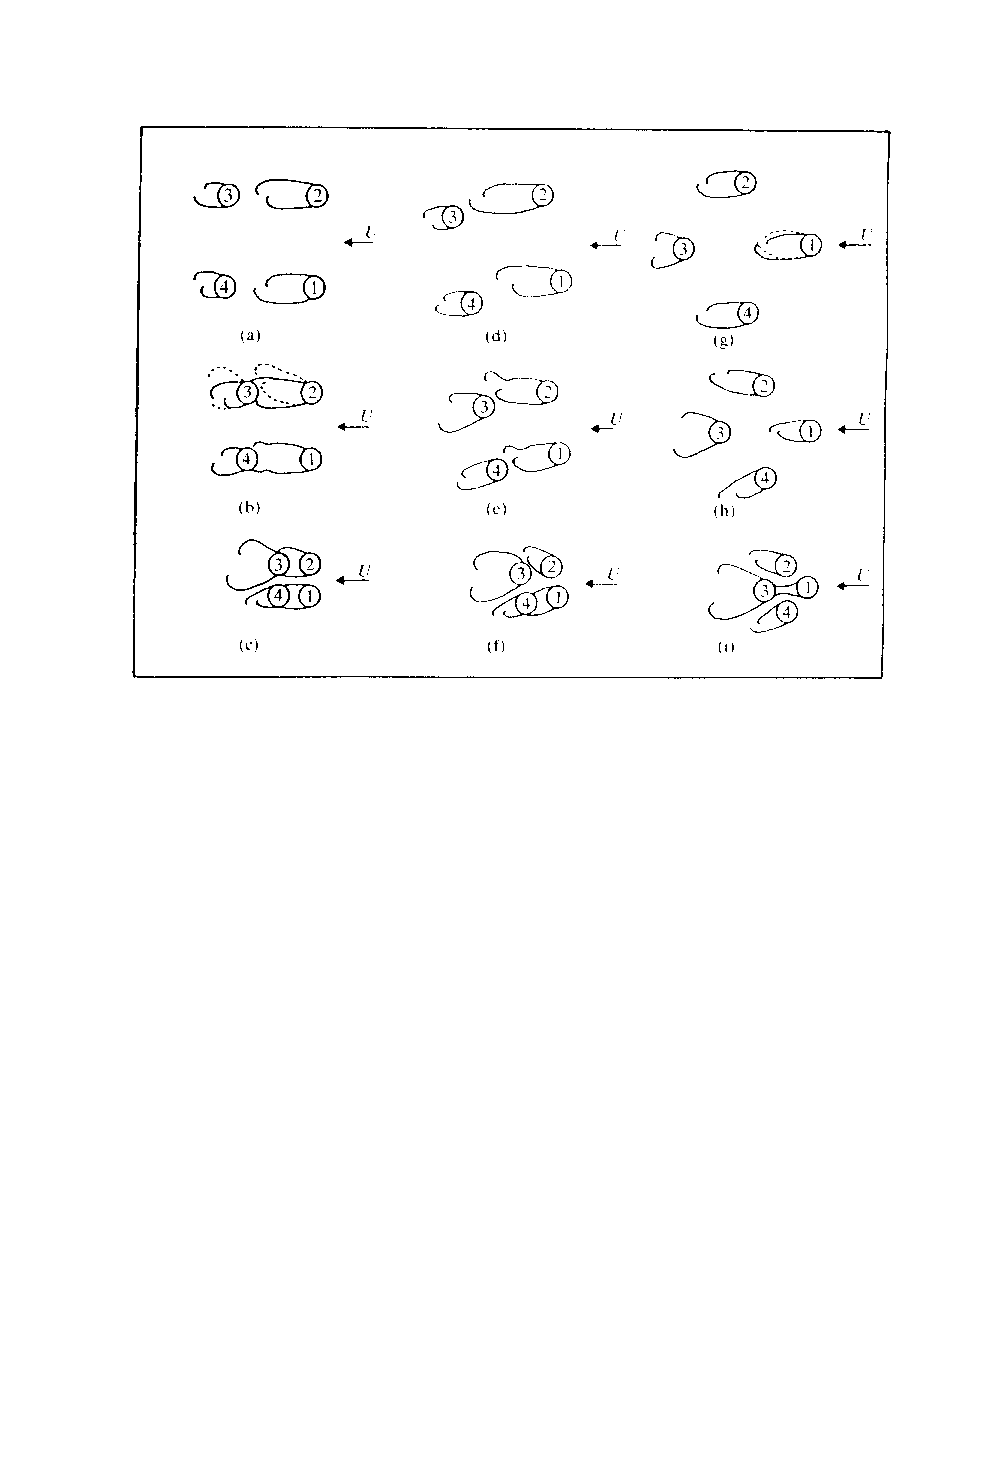
\includegraphics[width=0.7\linewidth]{Figs/visual4cylinders}
	\caption{Typical Row pattern in various arrangements (a) $ \theta = 0^\circ $, $ 3.94 < L_c/D $; (b) $ \theta = 0^\circ $, $ 1.70 < L_c/D < 3.94 $; (c) $ \theta=0^\circ $, $ L_c/D < 1.70 $; (d) $ \theta= 10^\circ $, $ 3.94< L_c/D  $; (e) $ \theta= 10^\circ $, $1.88< L_c/D <3.94$; (f) $ \theta= 10^\circ $, $ L_c/D < 1.88 $; (g) $ \theta= 20^\circ $, $ 2.40 < L_c/D $; (h) $ \theta= 20^\circ $, $ 1.28 < L_c/D < 2.40 $; (i) $ \theta= 20^\circ $. $ L_c/D = 1.28 $. $ L_c=$ centre to centre spacing ; $ \theta=$ flow incident angle.  \cite{Lam1992}}
	\label{fig:visual4cylinders}
\end{figure}

Compared with flow around two cylinders, cases with flow around cylinder arrays is more complicated and closer to the engineering reality (e.g.\ cylinder arrays in heat exchangers). On the whole, interaction between flow and multiple cylinders was sensitive to the cylinders' arrangement and the distance between each cylinder \cite{zhao2015flow}. This section summarises literature for both stationary \& elastically mounted cylinder arrays.

Four stationary cylinders in a square arrangement exposed to a steady flow have been investigated in many studies (e.g.\ see \Cref{fig:visual4cylinders}). The wake surrounding a four-cylinder array is much more complicated than that in previously mentioned one or two cylinders \cite{Lam2003}. It was experimentally found that \cite{Sayers1988}, at subcritical $ Re=30000 $, the orientation of the cylinder group (regarding the direction of inlet flow) had significant impact on drag and lift coefficients upon each cylinder. For both three and four equispaced cylinders, minor modifications in the cylinder group orientation can result in significant changes in vortex shedding frequency. Moreover, for certain combinations of spacing ratios and flow inclination angles, the vortex shedding can be asymmetrical or even absent \cite{Sayers1990}. Lam \& Lo \cite{Lam1992} carried out flow visualization studies in inline \& staggered square arrangements at subcritical $ Re=2100 $, and identified several distinct flow patterns (see \Cref{fig:visual4cylinders}). Furthermore, in subsequent studies \cite{lam1995effect, Lam2003, lam2003force}, the flow pattern was reported to have significant effects on the pressure distributions and the force coefficients. Flow patterns were found to change according to spacing ratios \cite{Lam2010,Lam2009}, meanwhile digital particle image velocimetry and numerical simulations were also applied to investigate this problem. For an inline arrangement, the vortex shedding mode was in-phase at small spacing ratios and anti-phase at large spacing ratios \cite{Farrant2000a}. Three types of flow patterns were found at $ Re = 200 $ \cite{Han2013}: when the spacing ratio is small, the wake flow resembles a single-bluff body flow pattern; when the spacing ratio is 1.6, wiggling shielding wake was observed; when the spacing ratio was 3.5-4.0, four vortex streets were observed. Three dimensional numerical simulations were carried out for an inline arrangement simulated \cite{Tong2014}. At a spacing ratio of 2 and $ Re=100 \sim 500 $, four flow regimes were distinguished and a significant effect on the force was discovered in transitions between the flow regimes.

\begin{figure}[tbp]
	\centering
	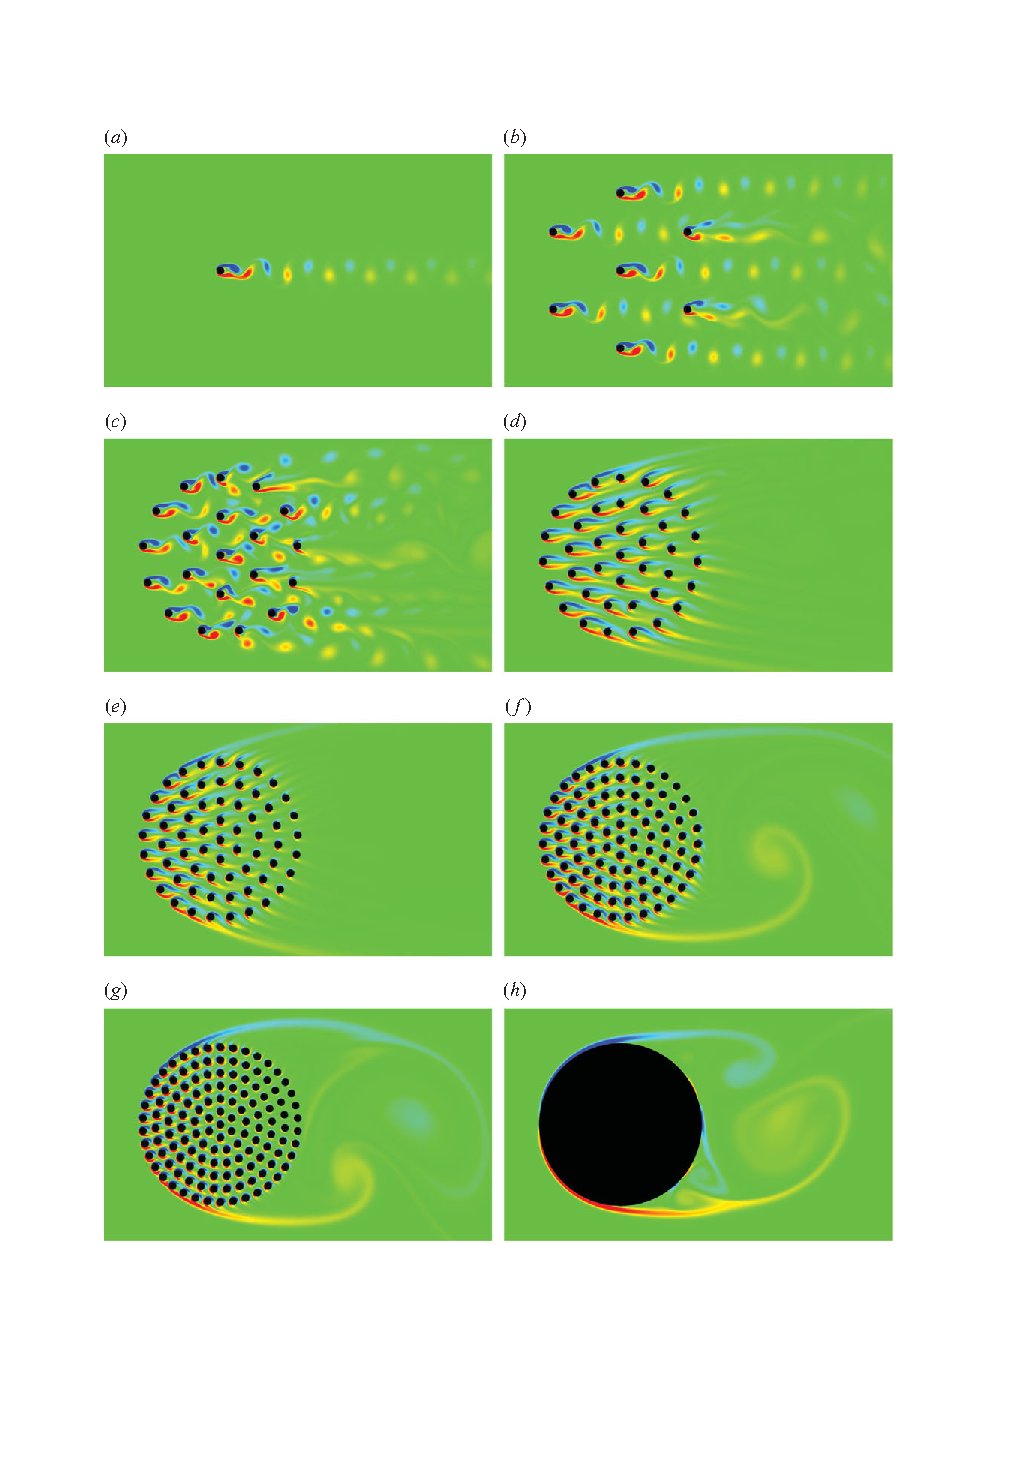
\includegraphics[height=1.3\textwidth]{Figs/multicylinders}
	\caption{Near field view of the vorticity field, $ \omega_v $, for the arrays (a) C1, (b) C7, (c) C20, (d) C39, (e) C64, (f) C95, (g) C133 and (h) CS1. $ Re=100 $ for C1 and $ Re=2100 $ for C7$ \sim $C133. The colours red and blue denote positive and negative vorticity respectively, with green corresponding to irrotational fluid. The flow is directed from left to right. \cite{Nicolle2011}}
	\label{fig:multicylinders}
\end{figure}

%Paper not available: Using wind tunnel experiments, Ball \& Hall \cite{ball1980drag} investigated square cylinder arrays for up to $ 9 \times 9 $ with different angles, and found that the flow incident angles influence the drag forces on the cylinders.

\begin{figure}[tbp]
	\centering
	\captionsetup{justification=centering}
	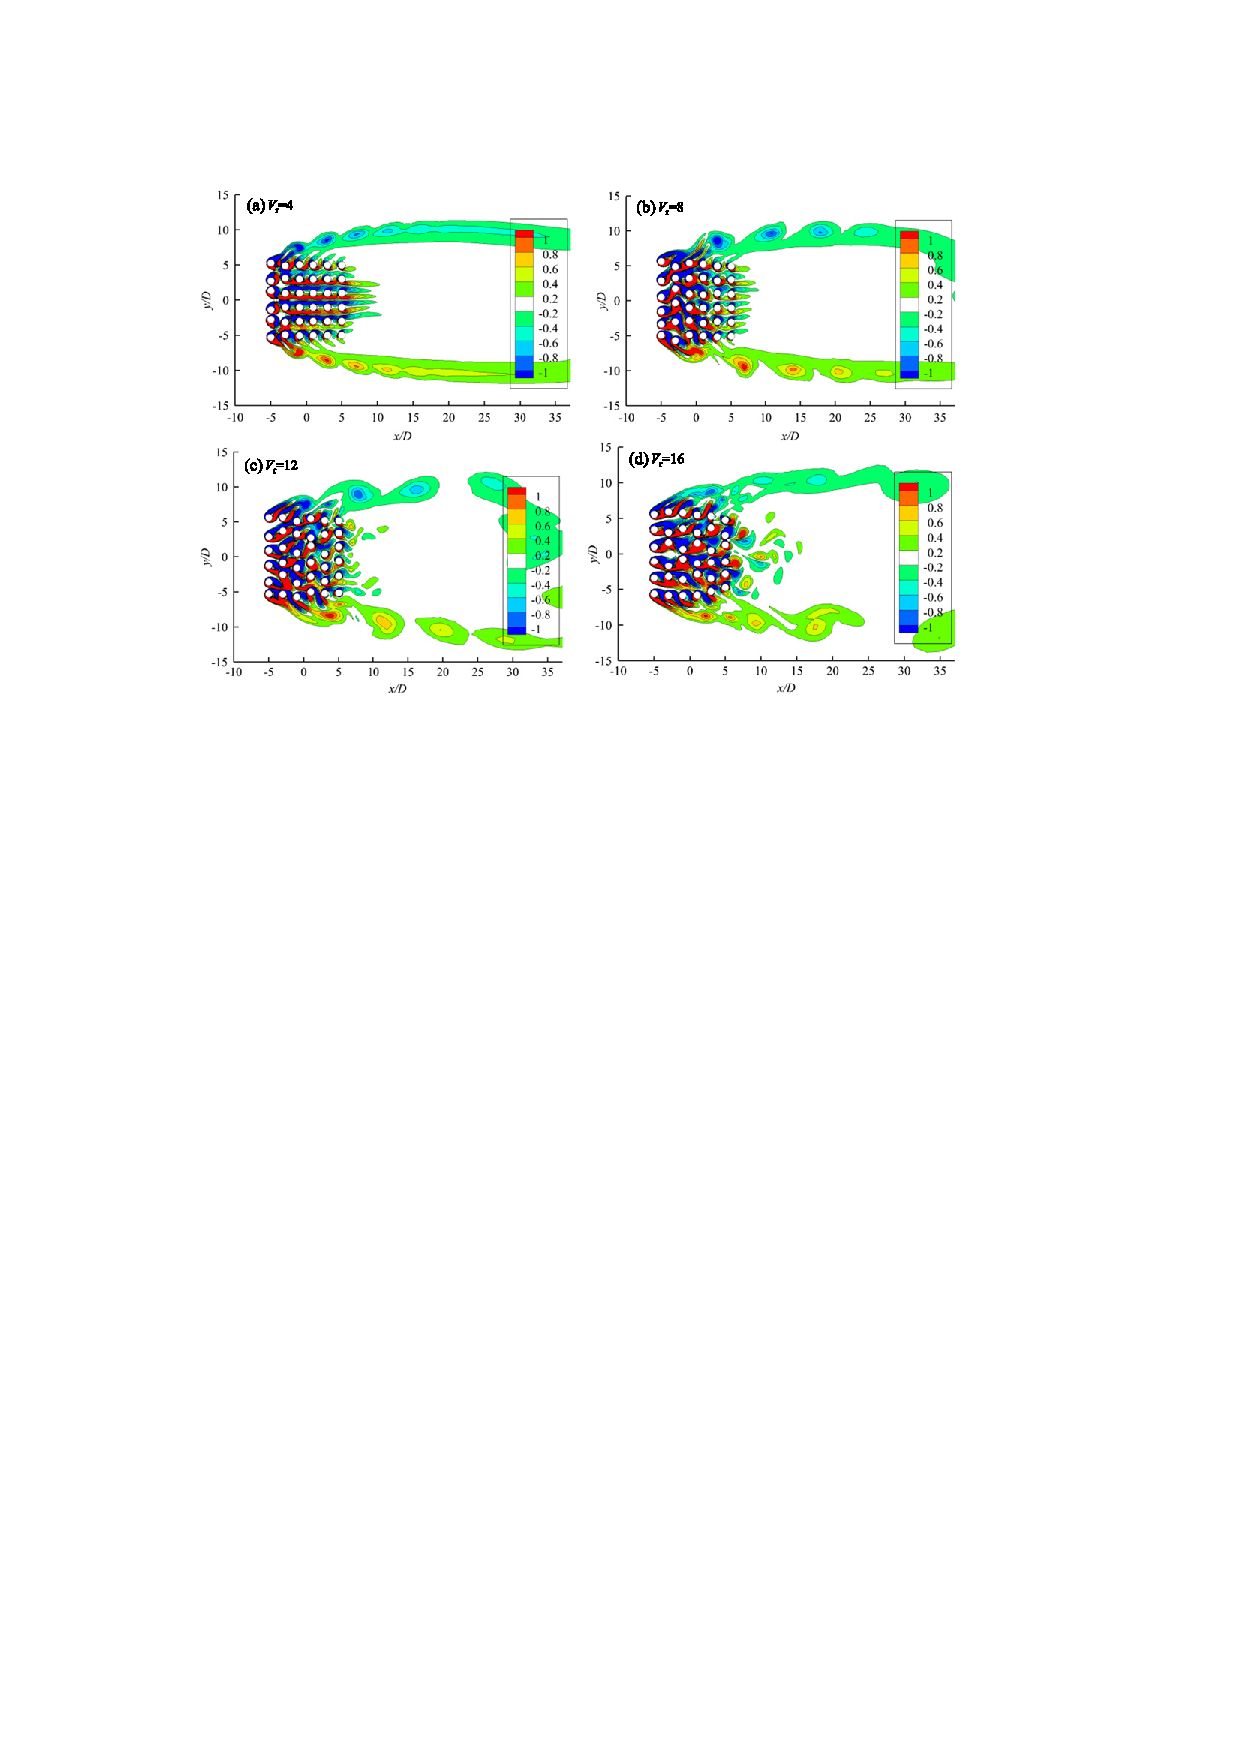
\includegraphics[width=0.9\linewidth]{Figs/VIVmulticylinderZhao}
	\caption{Contours of the non-dimensional vorticity for VIV of the cylinder array for $ L_c/D=2 $, $ Re=100 $, $ m^*=2.5 $. ($ L_c = $ centre-to-centre distance) \cite{Zhao2015b}}
	\label{fig:vivmulticylinderzhao}
\end{figure}

For stationary arrays with cylinder number $N >4 $ (e.g.\ see \Cref{fig:multicylinders}), greater complexity was encountered. Nicolle \etal{} \cite{Nicolle2011} carried out two-dimensional numerical simulations for arrays with $ 7 \sim 133 $ cylinders, and found that the flow field through and around the cylinder group had strong correlation with the void fraction $ \phi_v $ (i.e.\ indicating density of the cylinder group). As seen in \Cref{fig:multicylinders}, for sufficiently small void fractions ($ \phi_v <0.05$), the cylinders had uncoupled individual wake patterns, where the vorticity is rapidly dissipated by wake intermingling downstream. For moderate void fractions ($ 0.05< \phi_v <0.15$), the wake flow was stable and force on the cylinder array was steady. For high void fractions ($ \phi_v >0.15$), the wake behind the array was similar to a solid body of the same scale. Yu \etal{} \cite{Yu2013} simulated flow through a circular array of cylinders (similar to the configuration from Nicolle \cite{Nicolle2011}) in Reynolds numbers range 100 to 2000 using a hybrid RANS/LES turbulence model. They discovered that the drag coefficient increased with the void fraction, and was inversely correlated with Reynolds number. It was also found that the drag coefficient was independent of the cylinder array's diameter, when the void fraction and the Reynolds number were kept constant. Sweeney and Meskell \cite{Sweeney2003} developed a fast discrete vortex method to simulate flow past cylinder arrays at $ Re=2200 $. Their numerical result of Strouhal number was coherent with the previous data and the vortex shedding pattern qualitatively agreed with the flow visualization. The generation of three-dimensional vorticity was studied for flow past a square array of nine tubes with spacing ratios of 1.5 \cite{Kevlahan2005}. It was found that at $ Re =200 $ the three-dimensional instability was completely suppressed by tube's forced vibration, while at $ Re =1000 $ tube's forced vibration does not suppress the three-dimensional instability, yet the flow's spanwise correlation was increased and the Strouhal number for the two- and three-dimensional flows is about the same.

%Eames \etal{} \cite{Eames2004} developed a numerical model in order to analyse inviscid flow through groups of bodies, which was based on the definitions of Eulerian and Lagrangian mean velocities and their decompositions into near and far field components.

Flow-induced vibration for an array of cylinders has relatively limited number of studies compared with previous mentioned configurations. The investigation for VIV of multiple cylinders started with one flexible cylinder surrounded by rigid cylinders and later carried on to a stage that every cylinder is flexible. Price \etal{} \cite{Price1995} carried out experiments for a staggered array of several rows of rigid cylinders in air with one of them replaced by a flexible cylinder. They discovered that Strouhal numbers $ S $ did not change from one row to another, and $ S $ tended to increase as $ Re $ increases. Kevlahan \cite{Kevlahan2011} found that if a single cylinder with 1DOF in the transverse direction is surrounded by fixed cylinders (a common experimental configuration), the flow asymmetries caused by the movement of the central cylinder relative to its neighbours generates a "galloping" type instability in addition to the pure vortex-induced vibration of the isolated cylinder case. Kevlahan \cite{Kevlahan2011} also argued that the negative damping theory \cite{paiudoussis1988mechanisms} was inconsistent with the Navier-Stokes simulation results. Also, 1DOF configuration of the tube caused great overestimation of the critical velocity, while Navier-Stokes simulations which allow all tubes to move in 2DOF give results in good agreement with experiment. VIV of multiple cylinders with each of them having 1DOF was simulated numerically by Zhao \etal{} \cite{Zhao2015b}. They found that the vibration of the cylinders spread downstream with the increase of reduced velocity (see \Cref{fig:vivmulticylinderzhao}). The vibration amplitudes of the downstream cylinders peaked at higher reduced velocities than that of a single cylinder. The maximum possible response amplitudes occurred at the most downstream cylinders.

To summarise this section, most common configurations of multiple cylinders were the 4 cylinders in square arrangement (most often also inline), and circular arrays with more than 7 cylinders. All cases in the literature were subjected to steady flow, and the focus of the study was on the flow patterns. In other words, similar to studies for two cylinders, quantitative relationship between configurations (i.e.\ input) and results (i.e.\ output) for the cylinder arrays was not as well established as that for a single cylinder (see \Cref{sec:VIV1}), which was possibly due to a limited number of experiments (or simulations) and the complexity caused by the increase of the cylinder number. Also, as 2DOF simulation achieves better agreement with experiment \cite{Kevlahan2011}, further study can be carried out for cylinder array with 2DOF.


\section{Summary}

In summary of this chapter, although there have been numerous studies examining the VIV behaviour of elastically mounted cylinders and the flow patterns of stationary cylinders exposed to moving fluid, the effect of a circular cylinder-VIV induced by the vibration of another cylinder in stationary fluid, rather than flowing fluid, has never been examined in detail. In this study, the situation is simplified to the interaction between two rigid cylinders immersed in stationary fluid, where one cylinder undergoes forced harmonic vibrations to disturb the fluid while the second cylinder responds to this disturbance with 1DOF. This research aims to achieve a clearer understanding on how a vibrating cylinder (possibly the flow-induced vibration) exerts its influence on a nearby cylinder in still water, excluding the effects led by a water flow. This research mainly focuses on the sensitivity of the system behaviour to the initial gap ratios between the two cylinders, as well as the oscillating amplitude and the frequency of the active cylinder, whereas the non-dimensional mass ratio of both cylinders is kept constant as 2.5 and the specified vibration is at a low Reynolds number of 100. 
%
% \fi false
%%==============================
%
%
%\section{Notes}
%
%\begin{enumerate}
%	\item Compare flow pattern (v field, pressure field, vorticity) under different f1
%	\item Compare flow pattern of single and double cylinder
%	\item separation?
%	\item The flow reversal is primarily caused by an adverse pressure gradient imposed on the boundary layer by the outer potential flow. The streamwise momentum equation inside the boundary layer is approximately stated as
%	 \begin{equation}%\label{key}
%	 u{\partial u \over \partial s}=-{1 \over \rho }{dp \over ds}+{\nu }{\partial ^{2}u \over \partial y^{2}} 
%	 \end{equation}
%	 where 
%	 s
%	 y
%	 s,y are streamwise and normal coordinates. An adverse pressure gradient is when 
%	 d
%	 p
%	 d
%	 s
%	 0
%	 dp/ds>0, which then can be seen to cause the velocity 
%	 u
%	 u to decrease along 
%	 s
%	 s and possibly go to zero if the adverse pressure gradient is strong enough.
%	 \item mesh distortion: greater progression rates?
%	 \item If you want to draw the non-dimensional vorticity, you should divide AR by U/D  manually. 
%	 \item Streaklines are the loci of points of all the fluid particles that have passed continuously through a particular spatial point in the past. Dye steadily injected into the fluid at a fixed point extends along a streakline.
%	 \item \textbf{Pressure in a vortex}: The fluid motion in a vortex creates a dynamic pressure (in addition to any hydrostatic pressure) that is lowest in the core region, closest to the axis, and increases as one moves away from it, in accordance with Bernoulli's Principle. One can say that it is the gradient of this pressure that forces the fluid to follow a curved path around the axis.
%	 In a rigid-body vortex flow of a fluid with constant density, the dynamic pressure is proportional to the square of the distance r from the axis. In a constant gravity field, the free surface of the liquid, if present, is a concave paraboloid.
%	 In an irrotational vortex flow with constant fluid density and cylindrical symmetry, the dynamic pressure varies as P∞ − 
%	 K
%	 /
%	 r2
%	 , where P∞ is the limiting pressure infinitely far from the axis. This formula provides another constraint for the extent of the core, since the pressure cannot be negative. The free surface (if present) dips sharply near the axis line, with depth inversely proportional to r2. The shape formed by the free surface is called a hyperboloid, or "Gabriel's Horn" (by Evangelista Torricelli).
%	 The core of a vortex in air is sometimes visible because of a plume of water vapor caused by condensation in the low pressure and low temperature of the core; the spout of a tornado is an example. When a vortex line ends at a boundary surface, the reduced pressure may also draw matter from that surface into the core. For example, a dust devil is a column of dust picked up by the core of an air vortex attached to the ground. A vortex that ends at the free surface of a body of water (like the whirlpool that often forms over a bathtub drain) may draw a column of air down the core. The forward vortex extending from a jet engine of a parked airplane can suck water and small stones into the core and then into the engine.
%	 
%	 \item Pressure in a vortex[edit]
%	 
%	 The fluid motion in a vortex creates a dynamic pressure (in addition to any hydrostatic pressure) that is lowest in the core region, closest to the axis, and increases as one moves away from it, in accordance with Bernoulli's Principle. One can say that it is the gradient of this pressure that forces the fluid to follow a curved path around the axis.
%	 In a rigid-body vortex flow of a fluid with constant density, the dynamic pressure is proportional to the square of the distance r from the axis. In a constant gravity field, the free surface of the liquid, if present, is a concave paraboloid.
%	 In an irrotational vortex flow with constant fluid density and cylindrical symmetry, the dynamic pressure varies as P $ \infty $ − 
%	 K
%	 /
%	 r2
%	 , where P∞ is the limiting pressure infinitely far from the axis. This formula provides another constraint for the extent of the core, since the pressure cannot be negative. The free surface (if present) dips sharply near the axis line, with depth inversely proportional to r2. The shape formed by the free surface is called a hyperboloid, or "Gabriel's Horn" (by Evangelista Torricelli).
%	 The core of a vortex in air is sometimes visible because of a plume of water vapor caused by condensation in the low pressure and low temperature of the core; the spout of a tornado is an example. When a vortex line ends at a boundary surface, the reduced pressure may also draw matter from that surface into the core. For example, a dust devil is a column of dust picked up by the core of an air vortex attached to the ground. A vortex that ends at the free surface of a body of water (like the whirlpool that often forms over a bathtub drain) may draw a column of air down the core. The forward vortex extending from a jet engine of a parked airplane can suck water and small stones into the core and then into the engine.
%	 \item see \Cref{fig:tasunobearmankcbetaoriginal}, almost for all the cases with $ KC \leq 2$, if it is single cylinder oscillation, the flow patterns should be in the regime of $ A^* $. compare with the current case setup. 
%	 \item \textbf{Negative added mass} 
%	 
%	  \url{http://folk.ntnu.no/falnes/w_e/rpts_scnnd/added_mass_1983.pdf}
%	 
%	 ???????
%	 
%	 "A simple interpretation of the added mass would be to consider it as the mass of a lump of water which is pushed back and forth together with the oscillating body. However, even in a case where the added mass is zero water is pushed by the oscillating body. And it is evidently not correct to interpret a negative added mass as a 'subtracted mass' of water. Hence this interpretation is not physically correct. Negative added mass means that there is more potential energy than kinetic energy in the near field. 
%	 
%	 The correct interpretation of added mass is to attribute it to reactive power or to stored energy in the near field. This is analogous to the energy stored in a resonator." 
%	 
%	 \item \textbf{The occurrence of negative added mass in free-surface problems involving submerged oscillating bodies .pdf}:
%	 
%	 "multi-body problems the added mass takes the form of a matrix, reflecting the fact that the oscillations of one body can create a force on another. ... It is clear that a simple physical interpretation in terms of accelerated fluid mass is not appropriate in complicated multi-body problems where interaction effects are important."
%	 
%	 \textbf{Fluid-Structure Interactions: Cross-Flow-Induced Instabilities}:
%	 
%	 \textbf{P139}"Added mass in vortex-induced vibrations has been the subject of several controversies, resulting in some confusion on its physical meaning, its value and even its relevance. We focus now on some of the essential technical aspects behind these controversies to show similarities and differences between approaches, and hopefully, to clarify the situation. Several distinct issues have appeared when considering added mass in relation to VIV. Can added mass still be defined when VIV occurs? If so, is there any relation to its value in inviscid still fluid? What is the meaning of a negative added mass? Finally, what must be done in practice when computing the response of systems to VIV?"
%	 
%	 \textbf{P141}"As often emphasized, added mass in \textit{still} fluid is not the mass of a physical system. It is nevertheless always positive because it is the \underline{scaling factor of the kinetic energy of the fluid in relation with the solid motion} (see for instance de Langre 2002). Here, in the case of a \textit{moving fluid} with its own vorticity dynamics there is no a \textit{priori} reason that the force in phase with the acceleration should be opposite or in the same direction as the acceleration. In fact, as discussed below, the change in sign in added mass can be seen as the result of the dynamics of a wake oscillator."
%	 
%	 \item \textbf{Wake oscillator} 
%	 
%	 \url{http://www.sciencedirect.com/science/article/pii/S0889974603001853}
%	 
%	 The fluctuating nature of the vortex street is modelled by a nonlinear oscillator satisfying the van der Pol equation (Nayfeh, 1993)
%	 
%	 \item \url{http://www.fem.unicamp.br/~phoenics/SITE_PHOENICS/AULAS/GRADE%20&%20MALHA/annurev.fluid.36.050802.122128.pdf}
%	 	
%	 "We make the point here that added mass coefficients having a negative value can be observed in data sets collected from forced vibration (see Mercier 1973, Sarpkaya 1978, Gopalkrishnan 1993) and in recent free-vibration data sets (see Vikestad et al. 2000, Willden \& Graham 2001). The implications to free-vibration phenomena, such as the possible existence of a 'critical mass', were not deduced in these works. However, it has generally been recognized that added mass (or $ C_{EA} $ ) can predict free-vibration frequencies."
%	 
%	 \item \textbf{???}how did Viksted obtain total hydrodynamic force?
%	 
%	 \item Conclude: I should also investigate the added mass of the case, as there is currently no clear answer to this problem.
%	 
%	 \item In the case of a sinusoidal driving force:
%	 
%	 :$ \frac{\mathrm{d}^2x}{\mathrm{d}t^2} + 2\zeta\omega_0\frac{\mathrm{d}x}{\mathrm{d}t} + \omega_0^2 x = \frac{1}{m} F_0 \sin(\omega t),$
%	 
%	 where $\,\!F_0$ is the driving amplitude and $\,\!\omega$ is the driving [[frequency]] for a sinusoidal driving mechanism. This type of system appears in [[alternating current|AC]] driven [[RLC circuit]]s ([[Electrical resistance|resistor]]-[[inductor]]-[[capacitor]]) and driven spring systems having internal mechanical resistance or external [[air resistance]].
%	 
%	 The general solution is a sum of a [[Transient (oscillation)|transient]] solution that depends on initial conditions, and a [[steady state]] that is independent of initial conditions and depends only on the driving amplitude $\,\!F_0$, driving frequency, $\,\!\omega$, undamped angular frequency $\,\!\omega_0$, and the damping ratio $\,\!\zeta$.
%	 
%	 The steady-state solution is proportional to the driving force with an induced phase change of $\,\!\phi$:
%	 \begin{equation}%\label{key}
%	 x(t) = \frac{F_0}{m Z_m \omega} \sin ( \omega t + \phi)
%	 \end{equation}
%	 
%	 where
%	 
%	 \begin{equation}%\label{key}
%	 Z_m = \sqrt{\left(2\omega_0\zeta\right)^2 + \frac{1}{\omega^2}\left(\omega_0^2  - \omega^2\right)^2}
%	 \end{equation}
%	 is the absolute value of the [[Mechanical impedance|impedance]] or [[linear response function]] and
%	 \begin{equation}%\label{key}
%	 \phi = \arctan\left(\frac{2\omega \omega_0\zeta}{\omega^2-\omega_0^2 }\right)
%	 \end{equation}
%	 
%	 is the [[phase (waves)|phase]] of the oscillation relative to the driving force, if the arctan value is taken to be between -180 degrees and 0 (that is, it represents a phase lag, for both positive and negative values of the arctan's argument).
%	 
%	 For a particular driving frequency called the [[resonance]], or resonant frequency $\,\!\omega_r = \omega_0\sqrt{1-2\zeta^2}$, the amplitude (for a given $\,\!F_0$) is maximum. This resonance effect only occurs when $\,\zeta < 1 / \sqrt{2}$, i.e. for significantly underdamped systems. For strongly underdamped systems the value of the amplitude can become quite large near the resonance frequency.
%	 
%	 The transient solutions are the same as the unforced ($\,\!F_0 = 0$) [[damping|damped harmonic oscillator]] and represent the systems response to other events that occurred previously.  The transient solutions typically die out rapidly enough that they can be ignored.
%	 
%	 \item 
%	 
%\begin{figure}[tbp]
%	\centering
%	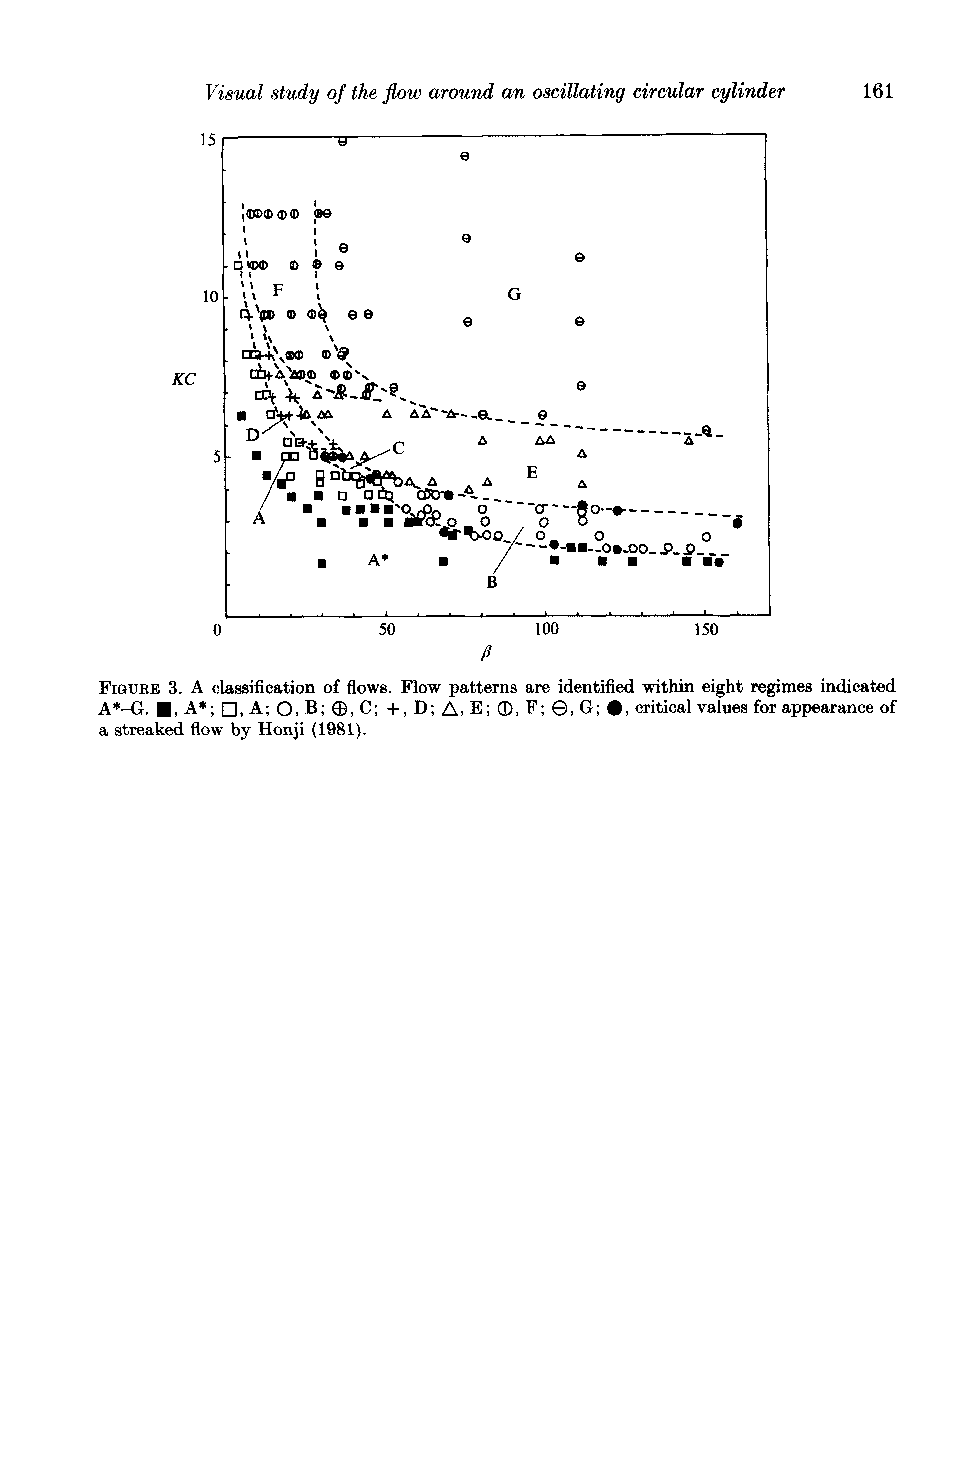
\includegraphics[width=0.7\linewidth]{Figs/tasunobearmanKCBeta_original}
%	\caption{}
%	\label{fig:tasunobearmankcbetaoriginal}
%\end{figure}
%	 
%\end{enumerate}
%
%\subsection{HYDRODYNAMIC PERFORMANCE OF AN ARRAY OF OSCILLATING WATER COLUMN DEVICE EXPOSED TO OBLIQUE WAVES}
%Wake vortex shedding topology of a cylinder undergoing vortex- induced vibrations (VIV) is investigated experimentally. Vibration measurements and flow visualization are utilized to study the con- nection between the cylinder response and the wake topology. The experiments were performed for two different orientations of the elliptic trajectories relative to the incoming flow at a fixed Reynolds number, moment of inertia ratio, mass ratio, and reduced velocity. Similar to the classical 2P regime, two counter- rotating vortex pairs are produced per oscillating cycle for both cases of elliptic trajectories examined here. However, significant changes in wake vortex dynamics are observed along the cylinder span. These changes include merging of vortices, which leads to shedding patterns similar to 2S and P þ S modes downstream of the vortex formation region. The observed changes in vortex dynamics are accompanied by splitting of spanwise vortex fila- ment and are attributed primarily to the changes in the local amplitude of vibrations along the span of the pivoted cylinder. It is shown that, being dependent on both the local amplitude of vibrations and vortex dynamics, the observed wake topology cannot be captured by the classical map of shedding regimes developed for VIV of one degree-of-freedom (DOF) cylinders. [DOI: 10.1115/1.4031971]



%CHECK REF:Blevins R 2001 Flow-Induced Vibration 2nd edn (Malabar, FL: Krieger)

%AGgreement and disagreement?

%Flow-induced vibration of elastically mounted cylinder arrays has also been investigated in depth by many scholars. VIV of single cylinder has been discussed extensively in \Cref{sec:VIV1}. 

%It has been widely acknowleged that 'lock-in' occurs over various regimes of reduced volocities, while the regime is determined by the mass
%REfer back to VIV single

%NO time, read only numerical and new articles





%? more water (non-compressible) than air (compressible) ? all the studies mentioned in the section are ... water?

%In summary, there are only limited number of experiments and there appears to be no justification that the results and conclusion from a certain condition (e.g.\ $ Re=2100 $) can be expanded to a range of other condions (e.g.\ $ Re=0\sim2100 $), which makes these results less practical for engineering applications, where $ Re $ is usually a function of time and space.
%Vortex-induced vibration of four cylinders in an in-line square configuration

%\section{Oscillation of single cylinder in still water}

%\section{Numerical simulation of high Reynolds number conditions}

%\section{Three-dimensional numerical simulation of VIV of cylinder in oscillatory flow}

%The results show that the 3-D numerical simulations have remedied the inadequacy of 2-D simulations and the results are in excellent agreement with the experimental results. \cite{Lam2010}


%============================================
%\nomenclature[z-]{}{}

%IFFALSE
%\iffalse 